%\listfiles
\documentclass[11pt]{article}
\usepackage{fullpage}
\usepackage{amssymb}
%\usepackage{a4}
\usepackage{fancyhdr}
\usepackage{subfigure}
\usepackage{ifthen}
\usepackage{version}
\usepackage{tocbibind}
\usepackage{makeidx}
%\usepackage{times}
\usepackage{booktabs}
\usepackage[colorlinks=true, pdfstartview=FitV, linkcolor=blue,
            citecolor=blue, urlcolor=blue]{hyperref}



%%%%%%%%%%%%%%%%%%%%%%%%%%%%%%%%%%%%%%%%%%%%%%%%%%%%%%%%%%%%
\input versioninfo.tex
%%%%%%%%%%%%%%%%%%%%%%%%%%%%%%%%%%%%%%%%%%%%%%%%%%%%%%%%%%%%

%%%%%%%%%%%%%%%%%%%%%%%%%%%%%%%%%%%%%%%%%%%%%%%%%%%%%%%%%%%%
\title{User Manual for \SplitsTree V\VERSION}
%%%%%%%%%%%%%%%%%%%%%%%%%%%%%%%%%%%%%%%%%%%%%%%%%%%%%%%%%%%%

%%%%%%%%%%%%%%%%%%%%%%%%%%%%%%%%%%%%%%%%%%%%%%%%%%%%%%%%%%%%
\author{Daniel H.~Huson and David Bryant}
%%%%%%%%%%%%%%%%%%%%%%%%%%%%%%%%%%%%%%%%%%%%%%%%%%%%%%%%%%%%

\raggedbottom
\sloppy

\parindent=0pt
\parskip=5pt

\makeindex

\input definitions.tex

\def\SplitsTree{{\sf SplitsTree4 }}
\def\kb{{\rm kb }}
\def\bp{{\rm bp }}
\def\Gb{{\rm Gb }}
\def\Mb{{\rm Mb }}

\def\this{.}

\ifx\pdfoutput\undefined
\usepackage[dvips]{graphicx}
\else
\usepackage[pdftex]{graphicx}
\fi


%%%%%%%%%%%%%%%%%%%%%%%%%%%%%%%%%%%%%%%%%%%%%%%%%%%%%%%%%%%%
\begin{document}
%%%%%%%%%%%%%%%%%%%%%%%%%%%%%%%%%%%%%%%%%%%%%%%%%%%%%%%%%%%%

\maketitle

\begin{center}
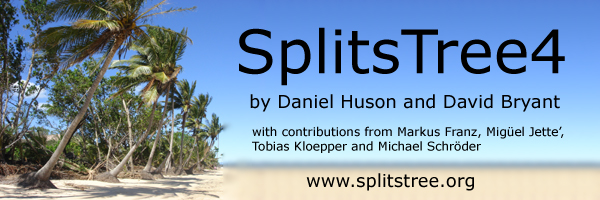
\includegraphics[height=3cm]{about.jpg}
\end{center}

\tableofcontents

%%%%%%%%%%%%%%%%%%%%%%%%%%%%%%%%%%%%%%%%%%%%%%%%%%%%%%%%%%%%
\mysection{Introduction}
%%%%%%%%%%%%%%%%%%%%%%%%%%%%%%%%%%%%%%%%%%%%%%%%%%%%%%%%%%%%

\ibf{License}:
Copyright (c) 2015, Daniel H. Huson and David J. Bryant

This program is free software: you can redistribute it and/or modify
it under the terms of the GNU General Public License as published by
the Free Software Foundation, either version 3 of the License, or
(at your option) any later version.

This program is distributed in the hope that it will be useful,
but WITHOUT ANY WARRANTY; without even the implied warranty of
MERCHANTABILITY or FITNESS FOR A PARTICULAR PURPOSE.  See the
GNU General Public License for more details.

You should have received a copy of the GNU General Public License
along with this program.  If not, see \url{http://www.gnu.org/licenses}.


\ibf{Type-setting conventions}:
In this manual we use e.g.\ {\tt Network}$\to${NeighborNet} to indicate
the {\tt NeighborNet} menu item in the {\tt Network} menu.
We use e.g.\ {\tt Main:Source} to indicate the {\tt Source} tab in the
{\tt Main} window.

\ibf{How to cite}:
If you publish results obtained in part by using \SplitsTree, then we
require that you acknowledge this by citing the program as follows:
\begin{itemize}
\item D.H. Huson and D. Bryant, {\em Application of Phylogenetic Networks
in Evolutionary Studies}, Molecular Biology and Evolution,
23(2):254-267, 2006.
software available from \url{www.splitstree.org},
\end{itemize}

Evolutionary relationships are usually represented using phylogenetic trees,
based on a model of evolution dominated by mutations and speciation
events. More realistic models must also account for gene genesis, loss and
duplication events, hybridization, horizontal gene transfer or
recombination. Here, phylogenetic networks have a role to play.

Moreover, network methods also provide a value tool for phylogenetic
inference even when reticulation events do not play an important role.
The combined effect of \pconcept{sampling error} and
\pconcept{systematic error} makes
phylogenetics an uncertain science, and network methods provide tools for
representing and quantifying this uncertainty.

The aim of \SplitsTree is to provide a framework for evolutionary
analysis using both trees and networks. The program takes as input
a set of taxa represented by characters (that is, aligned sequences),
distances, quartets, trees or splits and produces as output trees or
networks using a number of different methods.

This document provides both an introduction and a reference manual for
\SplitsTree.

\pagebreak
%%%%%%%%%%%%%%%%%%%%%%%%%%%%%%%%%%%%%%%%%%%%%%%%%%%%%%%%%%%%
\mysection{Getting Started}
%%%%%%%%%%%%%%%%%%%%%%%%%%%%%%%%%%%%%%%%%%%%%%%%%%%%%%%%%%%%

This section describes how to get started.

First, download an installer for the program from
from \href{http://www.splitstree.org}{www.splitstree.org},
see Section~\ref{sec:Obtaining and Installing the Program}
for details.

Use the \menuitem{File}{Open} menu item to open a file containing
data such as character sequences, distances or trees.
The file must be in one of the following formats:
\concept{Nexus}, \concept{ClustalW}, \pconcept{PhylipParsimony}, \concept{FastA} or
\pconcept{Newick}.
Alternatively, select the \menuitem{File}{Enter Data} menu item
 and enter data in one of these formats by hand.

Example files are provided with the program. They are contained in the
\itt{examples} sub directory of the installation directory. The precise
location of the installation directory depends upon your operating system.

Use the different menu items to determine which methods are applied
to the input data. The \menu{Distances}, \menu{Trees} and \menu{Network}
menus contain items that determine how to compute distances,
trees or a network from the given data. Some of the methods provided
have parameters that can be set using the
\menuitem{Analysis}{Configure Pipeline}
or
\menuitem{Analysis}{Configure Recent Methods} items.

The computed data can be viewed in text form in the \window{Data}
tab and can be saved using the \menuitem{File}{Save As} item.

The computed network or tree is displayed in the \window{Network}
tab. Attributes of the network can be changed by selecting nodes or branches
(also called edges)
and using the \window{Format Nodes and Edges} dialog which is reachable using
the \menuitem{View}{Format Nodes and Edges} item.

Individual blocks of data can be saved in a number of different
formats using the \menuitem{File}{Export} item.
The network displayed in the \window{Network} tab can
be saved in a graphics format using the \menuitem{File}{Export Image}
item.

%%%%%%%%%%%%%%%%%%%%%%%%%%%%%%%%%%%%%%%%%%%%%%%%%%%%%%%%%%%%
\mysection{Obtaining and Installing the Program}
%%%%%%%%%%%%%%%%%%%%%%%%%%%%%%%%%%%%%%%%%%%%%%%%%%%%%%%%%%%%

\SplitsTree is written in Java and requires a Java runtime environment
version 1.7 or newer, freely available from \href{http://www.java.org}{www.java.org}.

\SplitsTree is installed using an installer program that is freely available
from \href{http://www.splitstree.org}{www.splitstree.org}.
There are four different installers, targeting different operating systems:
\begin{itemize}
\item \itt{splitstree\_windows\_\VERSION.exe} provides an installer for \irm{Windows}.
\item \itt{splitstree\_macos\_\VERSION.dmg} provides an installer for \irm{Mac OS}.
\item \itt{splitstree\_unix\_\VERSION.sh} provides a shell installer for \irm{Linux}.
\end{itemize}

%%%%%%%%%%%%%%%%%%%%%%%%%%%%%%%%%%%%%%%%%%%%%%%%%%%%%%%%%%%%
\mysection{Program Overview}
%%%%%%%%%%%%%%%%%%%%%%%%%%%%%%%%%%%%%%%%%%%%%%%%%%%%%%%%%%%%

In this section, we give an overview over the main design goals
and features of this program. Basic knowledge of the underlying design of
the program should make it easier to use the program.

\SplitsTree is written in the programming language Java.
The advantages of this is that we can provide versions that run under the
\irm{Linux}, \irm{MacOS}, \irm{Windows} and \irm{Linux} operating systems.
Additionally, this makes it possible for the program to support plug-ins
that can add new functionality to the program, such as new methods
and import or export modules.
A potential draw-back is that an algorithm implemented in Java will generally
run slower than the same algorithm implemented in $C$ or $C{+}{+}$.

Earlier versions $1-3$ of the program \cite{SplitsTree98}
were written in $C{+}{+}$
and only contain a small part of what is now available with \SplitsTree.

\SplitsTree uses \irm{multi-threading} and supports \irm{multiple documents}.
This means that that you can work on more than one data set simultaneously,
in different windows, and run multiple calculations simultaneously,
making use of multiple processors, when available.

A \pconcept{Document} consists of an individual data set and possesses its own
\window{Main} window. The document is discarded, when its window is closed.
The program
is based on the \concept{Nexus} format, as introduced in
\cite{NEXUS} and the data associated with a document is organized into
\iem{blocks}, and each such block of data is represented by a corresponding
``block'' in the Nexus format. The blocks are:
\begin{itemize}
\item \block{Taxa}: the names of all taxa.
\item \block{Unaligned}: unaligned sequences.
\item \block{Characters}: aligned character sequences.
\item \block{Distances}: pairwise distances between taxa.
\item \block{Quartets}: (possibly weighted) quartet topologies.
\item \block{Trees}: list of (possibly partial) trees.
\item \block{Splits}: (possibly weighted) splits.
\item \block{Network}: phylogenetic tree or network.
\item \block{ST\_Assumptions}: contains all methods and options
used to compute data.
\item \block{ST\_Bootstrap}: bootstrap support of splits.
\end{itemize}

The first eight blocks \block{Taxa}, \block{Unaligned}, \block{Characters},
\block{Distances}, \block{Quartets}, \block{Trees}, \block{Splits}
and \block{Network} are organized as a \pconcept{pipeline} and data is processed
from left-to-right along this pipeline. Any non-empty document must contain
a \block{Taxa} block and will usually contain an \block{ST\_Assumptions}
block. All other blocks are optional and the presence or absence of
some block depends on the set of computations that the user has selected.

We will use the term \pconcept{source block} to denote the left-most block
in the pipeline (excluding the \block{Taxa} block). The source block
contains the original data that is provided to the program.
Any computations performed by the program will update blocks from left to
right along the pipeline, starting after the source block.
Note that some types of computations do not fit into this
pipeline design,  for example \SplitsTree cannot provide any method that
takes a \block{Splits} block and produces a \block{Trees} block, because
the latter occurs before the former in the pipeline.

Typically, the user will provide a source-block and
will then use different menu items to determine how the program will compute
data
along the pipeline until a \block{Network} block has been computed and
an image of the \concept{network} has been drawn in the
\window{Main} window.

The program is designed to keep all blocks in the pipeline \iem{synchronized}
by enforcing that the different blocks only contain data that
has been computed via the pipeline. For example, if you attempt
to load data from a file in \concept{Nexus} format that contains a
\block{Taxa} and two or more other blocks, e.g.\ a \block{Characters} block
or \block{Distances} block, then the program will request you to choose
which of the two latter blocks you want to keep. (This does not apply
if the file was created by \SplitsTree using the \menuitem{File}{Save}
or \menuitem{File}{Save As} command, in which case the blocks in the file
are synchronized, and so none must be discarded
and no computations are necessary).

Once a source block has been provided, the program will proceed
to perform a chain of \pconcept{default calculations}, which differ,
depending on the type of the source block.
In the case of a \block{Characters} block, the
program will use \method{UncorrectedP},
\method{NeighborNet} and then \method{EqualAngle} to compute a network for
the data. In the case of a \block{Distances} block,
\method{NeighborNet} and \method{EqualAngle} are used.
In the case of a \block{Trees} block, the first tree in the block is
displayed using the \method{EqualAngle} algorithm.

The data contained in the different blocks of the pipeline is displayed
in the \window{Data} tab.

The program is designed to operate in two differents modes:
in a GUI mode, the program provides a GUI for the user to interact with the
program. In \concept{command-line mode}, the program reads commands from a file
or from standard input and writes output to files or to standard output.

%%%%%%%%%%%%%%%%%%%%%%%%%%%%%%%%%%%%%%%%%%%%%%%%%%%%%%%%%%%%
\mysection{Splits, Trees and Networks}
%%%%%%%%%%%%%%%%%%%%%%%%%%%%%%%%%%%%%%%%%%%%%%%%%%%%%%%%%%%%

Here we give a brief introduction to some of the concepts
from phylogenetics that the program is based on.

Evolutionary relationships between taxa are usually represented using  a
phylogenetic \pconcept{tree}.
Such trees are often computed from molecular sequence
data, either directly, using methods such as parsimony, or indirectly,
by first computing a distance matrix and then applying a method such as
Neighbor-Joining.

Such approaches implicitly or explicitly model the evolution of a single
gene under the assumption that
the process is dominated by two types of events, mutations
and speciation events.
Under more complex models of evolution, i.e.\ involving gene loss and
duplication, or hybridization, horizontal gene transfer or recombination,
a single phylogenetic tree will often not be an appropriate representation
of the phylogentic history or of the different incompatible phylogenetic
signals. Also, the presence of noise in a data set, or uncertainty due
to inadequacies of the underlying model up on which a tree inference is
based, may also make it necessary to use a more general graph,
that is, a \pconcept{network}, to represent the data.

The aim of \SplitsTree is to provide a frame-work for computing phylogenetic
networks. As the name of the program suggests, it is based on the
fundamental mathematical concept of a \pconcept{split}.
For example, if we are given an alignment of binary sequences
\begin{verbatim}
a 010011010110
b 100001011110
c 011001101110
d 010001101111
\end{verbatim}
then each non-constant column in the alignment defines a split of the taxon set
consisting of those taxa with the value $0$ and those with the value $1$.
For example,
the first column partitions the taxa into two sets $\{a,c,d\}$  and  $\{b\}$,
and thus gives
rise to the split $\frac{\{a,c,d\}}{\{b\}}(=\frac{\{b\}}{\{a,c,d\}})$,
while the fourth
column does not define a split because the characters are constant.

Mathematically, for a set of $X$ taxa any phylogenetic tree $T$ defines a set
of such splits called the \pconcept{split encoding} $\Sigma(T)$ of $T$, as
follows:
deletion of any \pconcept{branch} (also called \pconcept{edge}) $e$ in the
tree produces two subtrees, $T_A$ and $T_B$,
say, and they give rise to a split $S=\frac{A}{B}=\frac{B}{A}$,
consisting of the set $A$ of all taxa contained in $T_A$ and the set $B$
of all taxa contained in $T_B$. In the literature, a split $\frac{A}{B}$ is sometimes denoted
by $A|B$ or $\{A,B\}$.

For example, consider the tree $T$ displayed in Figure~\ref{fig:splitsexample}.
Its split encoding $\Sigma(T)$ contains $5$ \pconcept{trivial splits}
that separate a single taxon from all other taxa, and $2$
\pconcept{non-trivial splits} that contain at least two taxa in both parts.
The trivial splits are:
$$
\frac{\{a\}}{\{b,c,d,e\}},
\frac{\{b\}}{\{a,c,d,e\}},
\frac{\{c\}}{\{a,b,d,e\}},
\frac{\{d\}}{\{a,b,c,e\}} \mbox{~and~}
\frac{\{e\}}{\{a,b,c,d\}},
$$
and the non-trivial ones are:
$$
\frac{\{a,b\}}{\{c,d,e\}} \mbox{~and~}
\frac{\{a,b,e\}}{\{c,d\}}.
$$

\begin{figure}[ht]
\begin{center}
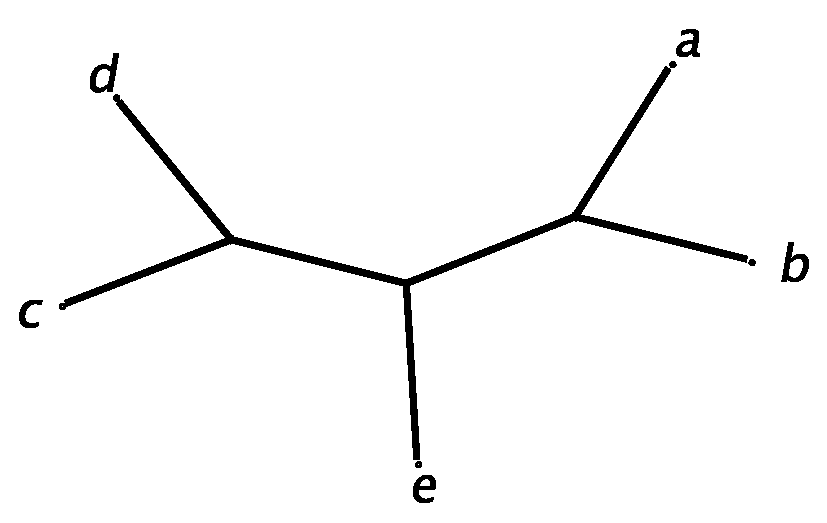
\includegraphics[height=3cm]{splitsexample.pdf}
\end{center}
\caption{An unrooted phylogenetic tree.}\label{fig:splitsexample}
\end{figure}

A fundamental result in mathematical phylogeny states that
any given set of splits $\Sigma$ corresponds to some phylogenetic tree $T$,
with $\Sigma(T)=\Sigma$, if and only if $\Sigma$ is
\pconcept{compatible} \cite{buneman.dist}.
Thus, any phylogenetic tree may be viewed as a graph whose task it
is to give a visual representation of a given set of compatible splits.


A phylogenetic tree can be thought of as an idealized representation of the
historical relationships among a set of taxa; and tree building methods are
attempts to find a the set of compatible splits that are most consistent with
the data according to some algorithm.  Often there are multiple tree that are
equally consistent with the data, i.e.\ multiple sets of compatible splits.  In
general that collection of splits will be incompatible.  Moreover, there exist
inference methods such as \concept{split decomposition} and
\concept{Neighbor-Net} that compute a
set of incompatible splits from the data in the form of a given distance
matrix.  Note that split decomposition produces a set of splits that are called
\pconcept{weakly compatible}, while Neighbor-Net produces a set of splits that
is \pconcept{circular}, as originally defined in \cite{BandeltDress92}.

A \pconcept{split network} is a more general type of phylogenetic graph
that can represent any collection of splits, whether incompatible or not
\cite{BandeltDress92}.
For a compatible set of splits, it is always possible to represent
each split by a single \concept{branch}, and thus the resulting graph is a
tree.
In general, however, this will not be possible and in a split network
usually a whole band of \pconcept{parallel branches} (also called
\pconcept{parallel edges}) is required to represent a single
split. A phylogenetic tree is therefore a special case of a split network.
In \SplitsTree, if you click on any branch in the representation of
a split network, then all branches corresponding to the same split will be
highlighted. If one were to delete all branches corresponding to a given split
$S$, then the remaining graph will consist of precisely two components,
$G_{A}$ and $G_{B}$, and, as above, the we have $S=\frac{A}{B}$, where
$A$ is the set of all taxa contained in $G_{A}$ and $B$ is the set of all
taxa contained in $G_{B}$.

\ignore{
There is an important difference between phylogenetic trees
and more general split networks: Any rooted tree has a direct
interpretation in evolutionary terms: the leaves represent taxa and the
internal nodes represent speciation events.
In a (possibly rooted) split network, the internal nodes do not have such a
direct interpretation. Instead, split networks must be viewed on a more
abstract level as networks giving a visual representation of incompatible
signals, that is, showing how ``tree-like'' or ``certain'' parts of a
phylogeny are.

A \pconcept{ network} is used to describe
\pconcept{reticulate evolution} and there are two types of such networks,
one is the \pconcept{hybridization network}
and the other is the \pconcept{recombination network}.
A hybridization network describes evolution in the presence of
\pconcept{hybridization} events such as
\pconcept{allopolyploidization} or \pconcept{diploid} hybridization,
and in both cases the net effect is that a new species arises that
has obtained some of its genes via one ancestral species and the other
genes via another ancestral species.
A recombination network
is used to describe evolution in the presence of \pconcept{recombination}
events.
As presently implemented in \SplitsTree, such recombination networks can
only be computed for \pconcept{binary} sequences. Such sequences may, for
example,
indicate the presence or absence of a certain restriction site at a certain
position.
There are two main  differences between hybridization networks and
recombination networks. First, the former are based on gene trees, whereas the
latter are based on sequences. Second, a recombination network is
additionally annotated by inferred sequences at each of the nodes
and the mutations that happen along each of the branches. Moreover,
the recombination nodes are usually annotated with a description of
which parts of the two ancestor sequences are used in the recombination
event.

In contrast to split networks, these types of networks can be
directly interpreted in evolutionary terms.
Recent research has revealed that there are strong connections between
split networks and reticulate networks
\cite{Reticulate2005,HusonKloepper2005}
and these are used in \SplitsTree to provide methods for computing
reticulate networks.
}
% ??? Add papers that discuss the application of such methods:

A more detailed discussion of the fundamental concepts can be found in
\cite{jsplits} and \cite{Tutorial2005}.


%%%%%%%%%%%%%%%%%%%%%%%%%%%%%%%%%%%%%%%%%%%%%%%%%%%%%%%%%%%%
\mysection{Opening, Reading and Writing Files}
%%%%%%%%%%%%%%%%%%%%%%%%%%%%%%%%%%%%%%%%%%%%%%%%%%%%%%%%%%%%

To open a file, select the \menuitem{File}{Open}
menu item and then browse to the desired file. Alternatively, if the file
was recently opened by the program, then it may be contained in
the \menuitem{File}{Open Recent} submenu.

The native file format of \SplitsTree is based on the \concept{Nexus} format,
see \cite{NEXUS}.
However, the program can also parse a number of other formats, including
\concept{ClustalW} format for aligned sequences,
\concept{Phylip} format for sequences and distances, \concept{FastA} format for aligned
distances and \concept{Newick} format for trees. Earlier versions had separate Open and Import menu items; these have now been combined.

If a file is opened while the \window{Network} tab or
\window{Data} tab is open,
then the program will attempt to parse and execute the file.
If the file is a complete Nexus file previously generated by \SplitsTree, then
the network described in the file will be displayed.
If the file is in some other format, then, depending on the type of content,
the program will perform a chain of \concept{default calculations}.

To save the complete data associated with a given window in \SplitsTree's
native Nexus format, use the \menuitem{File}{Save}
or \menuitem{File}{Save As} menu items.
To save selected blocks of data, or to export data in a different
file format, use the \menuitem{File}{Export}.
A picture of the computed \concept{network} can be saved using
the \menuitem{File}{Export Image} menu item.

%%%%%%%%%%%%%%%%%%%%%%%%%%%%%%%%%%%%%%%%%%%%%%%%%%%%%%%%%%%%
\mysection{Estimating Distances}
%%%%%%%%%%%%%%%%%%%%%%%%%%%%%%%%%%%%%%%%%%%%%%%%%%%%%%%%%%%%

Many methods in phylogenetics begin by estimating distances between the
taxa. This is done by
taking sequences two at a time and estimating the average number of mutations
that occurred on the paths from them to their most recent common ancestor. If
the rate of mutation was constant, then this will be proportional to their
divergence time. \SplitsTree provides a large number of methods for estimating
distances, for sequences and other types of data.

The \method{UncorrectedP} method computes the proportion of positions at
which two
sequences differ. For DNA or RNA sequences, there are choices over how ambiguous
state codes (such as W, M, V) are handled. Ignore, means that these states are
treated as missing states.  'Average' means that the contribution at a site is
averaged over all possible resolutions of the ambiguous codes, with the
exception that sites having the same ambiguous code contribute zero. 'Match'
looks at each possible state in each sequence, counts one if the state is not a
possible resolution of the ambiguous code in the other sequence, and normalises
the count by the number of states for each ambiguous code.


The \menu{Distances} menu lists several standard distance
estimation methods. Most of these have parameters that can be changed.
When you select the menu item the \window{Pipeline} window will open
and will display a panel for setting the parameters of the method.
If you always use the same parameters for a given method, or if the method
has no parameters, then
selecting the ``Don't show this dialog to configure this method again''
will prevent the  dialog from appearing again.
All methods can be configured using the \window{Pipeline} window, accessed by
\menuitem{Analysis}{Configure Pipeline} or
\menuitem{Analysis}{Configure Recent Methods}.

%%%%%%%%%%%%%%%%%%%%%%%%%%%%%%%%%%%%%%%%%%%%%%%%%%%%%%%%%%%%
\mysection{Building and Processing Trees}
%%%%%%%%%%%%%%%%%%%%%%%%%%%%%%%%%%%%%%%%%%%%%%%%%%%%%%%%%%%%

The \menu{Trees} menu provides a number of methods for constructing trees,
both from distance and character data.
The following distance-based methods are available:
\method{NJ}, \method{BioNJ}, \method{UPGMA},
\method{BunemanTree} and \method{RefinedBunemanTree}.

The program provides `front-ends' for several tree based programs,
currently \method{PhyML} and
\method{PhylipParsimony}. \SplitsTree will pass these programs
the current sequences,
and place any trees produced in the \SplitsTree \block{Trees} block.
Our distribution of \SplitsTree does not provide any external programs, so
you must install them separately.
\ignore{
The first time an external application is used, or if an external
application cannot be found, then
\SplitsTree will bring up a dialog box asking you to locate
the application.
}
In the dialog that is associated with such a method you must
specify the location of the external application, e.g.~ using
the \itt{PhyML Path} text field. Once entered, the program will remember
this entry as the default value.

\SplitsTree provides a number of methods for processing a collection of
trees. The \menuitem{Trees}{TreeSelector} menu contains items to select
individual trees or to compute a consensus of trees.
If the \menuitem{Trees}{TreeSelector} is selected, then
the \menuitem{Trees}{Previous Tree} and
\menuitem{Trees}{Next Tree} items can be used to move from one tree to the
next in the \block{Trees} block.
Pressing the shift-key when selecting either of these methods will
move to the first tree, or the last tree,
respectively.
The \menuitem{Trees}{ConsensusTree} can be used to compute the majority or
strict consensus tree.

As with distances,
when you select such a menu item the \window{Pipeline} window will open
and will display a panel for setting the parameters of the method.
If you always use the same parameters for a given method, or if the method
has no parameters, then
selecting the ``Don't show this dialog to configure this method again''
will prevent the  dialog from appearing again.
All methods can be configured using the \window{Pipeline} window, accessed by
\menuitem{Analysis}{Configure Pipeline} or
\menuitem{Analysis}{Configure Recent Methods}.

%%%%%%%%%%%%%%%%%%%%%%%%%%%%%%%%%%%%%%%%%%%%%%%%%%%%%%%%%%%%
\mysection{Building and Drawing Networks}
%%%%%%%%%%%%%%%%%%%%%%%%%%%%%%%%%%%%%%%%%%%%%%%%%%%%%%%%%%%%

The \menu{Network} menu provides methods for computing phylogenetic
networks from character sequences, distances and trees.

Methods that compute a \concept{split network} directly from character sequences
provided in the \block{Characters} block
are \method{ParsimonySplits}, \method{MedianNetwork} , \method{MedianJoining}
and
\method{SpectralSplits}.
Note that the Median network method requires binary sequences.
However, given DNA or RNA, this program will detect all sites that contain
precisely two character-states and will build a Median network from these.

The MedianJoining method computes an unrooted network from
binary sequences, DNA and other multi-state sequences.
This is an implementation of the algorithm described
in \cite{Bandelt1999}.
In the case of non-binary sequences, the resulting network will not
be a split network.

Two methods for computing split networks from distances provided
in the \block{Distances} block are
\method{SplitDecomposition} and \method{NeighborNet}.

If a set of phylogenetic trees in the \block{Trees} block
all contain the full set of taxa listed in the \block{Taxa} block,
then the \method{ConsensusNetwork} method can be applied
to compute a \irm{consensus network}.
If, however, the \block{Trees} block contains \irm{partial trees}, that is,
trees that do not necessarily all involve identical sets of taxa,
then the \method{SuperNetwork} or \method{FilteredSuperNetwork}
method can be used to compute a \irm{super network}.

\ignore{
The \menu{Network} menu also provides two methods for computing \iem{reticulate
networks}. If the \block{Trees} block contains more than one tree,
then the \method{HybridizationNetwork} method can be used to
compute a \iem{hybridization network} for the given data set.
More precisely, the \method{HybridizationNetwork} requires that the
\block{Trees} and
\block{Splits} blocks are present and non-empty.
If the \block{Characters} block contains binary sequence data,
then the \method{RecombinationNetwork} method can be used to
compute a \iem{recombination network}.
}

The {\em Draw} menu determines which algorithm is used
to construct the final visualization of the \concept{tree} or
\concept{network}.
Existing methods
are \method{EqualAngle}, \method{RootedEqualAngle} and  \method{Phylogram}.
\ignore{
and \method{ReticulateNetwork}.
}
Additionally,  the \menuitem{Draw}{Hide Selected Splits} can be used to
remove selected splits from the network and the
\menuitem{Draw}{Select Trees} can be used to highlight different trees
contained in a split network.

%%%%%%%%%%%%%%%%%%%%%%%%%%%%%%%%%%%%%%%%%%%%%%%%%%%%%%%%%%%%
\mysection{Main Window}
%%%%%%%%%%%%%%%%%%%%%%%%%%%%%%%%%%%%%%%%%%%%%%%%%%%%%%%%%%%%

With \SplitsTree, multiple documents can be opened and worked on
simultaneously. Each document is represented by a \window{Main} window.
Additional
windows or dialogs are sometimes opened to perform certain tasks.

The \pwindow{Main} window is split vertically into two panels:
\begin{itemize}
\item the left-hand \window{Data} panel is used to display  all data associated
with a given document in text format, and
\item the right-hand \window{Network} panel contains the current tree or network.
\end{itemize}

We now discuss each separately:

\mysubsection{Network Tab}

The \pwindow{Network} tab is used to display the computed tree or network.
A \concept{status line} of text along the bottom of the network pane gives a
summary of the data, such as number of taxa, length of sequences, etc, and
a summary of the methods used to compute the network.
Optionally, a \concept{scale bar} can be displayed in the upper left
corner of the Network-tab to indicate the scale of branches.
The scale bar is can be turned on or of using the
\tab{Preferences}{General} tab.
The scale bar can be configured using the
\tab{Preferences}{Status Line} tab.

\mysubsection{Data Tab}

The \pwindow{Data} tab provides a textual display of the data associated with
the given document in the program's native \concept{Nexus} format, organized in a
linear list of items that can be either collapsed or expanded.
This view of the data is read-only.


\mysubsection{Tool bar}

The \concept{tool bar} associated with the window provides buttons for quick access to
many of the menu items. It can be configured using the
The \tab{Preferences}{Toolbar} tab.


%%%%%%%%%%%%%%%%%%%%%%%%%%%%%%%%%%%%%%%%%%%%%%%%%%%%%%%%%%%%
\mysection{Graphical Interaction with the Network}
%%%%%%%%%%%%%%%%%%%%%%%%%%%%%%%%%%%%%%%%%%%%%%%%%%%%%%%%%%%%

We now describe how the user can interactively modify the layout and
attributes of the displayed \concept{network}.
The \menu{View} menu
is used to rotate, move, and zoom in and out. Alternatively,
the view can be changed
using a wheel mouse, together with the following modifier keys:

\begin{center}
 \begin{tabular}{l|l}
 \hline
 none &   zoom in and out.\\
 Shift & rotate \\
 ALT/option & move vertically \\
 Shift \& ALT/option  & move horizontally \\
\hline
\end{tabular}
\end{center}

Here are additional modifications that can be performed:
\begin{itemize}
\item The graph can be dragged around by clicking and dragging a node.
\item If all selected nodes lie on one side of a band of
\concept{parallel branches} representing a single split, then clicking and
dragging on one of the nodes will change
the angle of the branches.
\item
By default, clicking on an edge will select {\em all}
edges representing the same
split, and all nodes on the smaller side of the represented split.
To select all nodes on the other side of the split,
use the \pmenuitem{View}{Invert Selection} menu item.
To allow selection of individual edges,
deselect the \itt{Split-Selection Mode} check box in the
\tab{Preferences}{General} tab.
\item Select a node by clicking on it. Press the mouse button
  outside of the network and drag  a
rectangle to select several nodes at once. Hold the shift key and click to add
or remove further nodes from the set selected.
\item Click on a text label to edit it.
\item Double-click on an edge to edit its label.
\item By default, node labels are automatically positioned to avoid overlap.  Any label that has been interactively reposition by the user is no longer automatically positioned.
To apply automatic positioning all node labels, including those that have been
moved by the user, deselect and then select
the \menuitemh{View}{Node Label Layout}{No Overlaps} check box.
\item Many aspects of the visual representation of nodes and edges can be
modified
using the \window{Format Nodes and Edges} window, which is opened using the
\menuitem{View}{Format Nodes and Edges} menu item.
\end{itemize}

%%%%%%%%%%%%%%%%%%%%%%%%%%%%%%%%%%%%%%%%%%%%%%%%%%%%%%%%%%%%
\mysection{Main Menus}
%%%%%%%%%%%%%%%%%%%%%%%%%%%%%%%%%%%%%%%%%%%%%%%%%%%%%%%%%%%%

We now discuss all menus of the \window{Main} window.

%%%%%%%%%%%%%%%%%%%%%%%%%%%%%%%%%%%%%%%%%%%%%%%%%%%%%%%%%%%%
\mysubsection{File Menu}

The \pmenu{File} menu contains the usual file-related items:
\begin{itemize}
\item
The \pmenuitem{File}{New} item opens a new \window{Main} window.
\item
The \pmenuitem{File}{Open} item provides an \window{Open File} dialog
to open a file containing input data in one of the supported formats.

If the file contains character sequences, then the program must know whether
the sequences are DNA, RNA, protein or ``standard'' (0,1) data.
In \concept{Nexus} files, the \irm{datatype} is explicitly given.
In other file formats
this not always the case. If the program cannot guess the \irm{data type}
(e.g., if all character states are 'A'), then the program will display
a \window{Choose Datatype} dialog and prompt the user to specify the data
type.

If the current document is non-empty, then the selected file
is opened in a new \window{Main} window.
\item
The \pmenuitem{File}{Open Recent} submenu provides access to recently
opened or saved files.
\item
The \pmenuitem{File}{Replace} item is used to replaced the current
data by a new data set.
\item
The \pmenuitem{File}{Clone} item clones the current window.
\item
The \pmenuitem{File}{Enter Data} item opens the \window{Data Entry} dialog, which can be used to enter data by hand (or copy-and-paste)
in a number of different formats.
\item
The \pmenuitem{File}{Close} item closes the current document.
\item
The \pmenuitem{File}{Save} item saves the current document to its file, if known.
\item
The \pmenuitem{File}{Save As} item provides a \window{Save As} dialog
and saves the current document to selected file.
\item
The \pmenuitem{File}{Export} item opens the \window{Export} dialog
which is used to save individual data in a number of different
formats.
\item
The \pmenuitem{File}{Export Image} item opens the \window{Export Image} dialog
which is used to save the current network in a number of different
formats.
\item The \pmenuitem{File}{Tools} item provides a submenu of tools.
The \pmenuitemh{File}{Tools}{Load Trees} item can be used to
\irm{merge a set of trees}
into one document. This item opens a dialog for opening
multiple files. The program parses all given files and extracts any trees found
in them and opens a new \concept{Document} containing all trees found.
The \pmenuitemh{File}{Tools}{Load Multi-Labeled Tree} item can be used to
read a single tree containing multiple labels and to convert it into
a single-labeled split network (and will be made available upon publication of
the paper describing this new method).
The \pmenuitemh{File}{Tools}{Concatenate Sequences} item can be used to
\irm{concatenate sequences} from different files
into one document. It requires that each of the input files uses exactly the
same set of taxon labels.
The \pmenuitemh{File}{Tools}{Group Identical Haplotypes} tools is used to detect multiple identical sequences or taxa. These are recognised from  the \block{Characters} or, if there is no \block{Characters} block, from the distances block. Only selected sites are used to test if two taxa are distinguishable. A new document is created; identical taxa are collapsed into a single taxa with label 'TYPEx'  (x ranging from $1,2,3,\ldots$, and the original taxa stored in the info field of the \block{Taxa} block. Note that files with hundreds or thousands of identical sequences can cause SplitsTree to stall. One solution is to cancel the computations after data is read in,
and to then use this tool to create a new smaller document containing only distinct sequences.
\item
The \pmenuitem{File}{Print} item is used to print the current network.
\item
The \pmenuitem{File}{Quit} item quits the program, after asking whether
to save unsaved changes.
\end{itemize}

%%%%%%%%%%%%%%%%%%%%%%%%%%%%%%%%%%%%%%%%%%%%%%%%%%%%%%%%%%%%
\mysubsection{Edit Menu}

The \pmenu{Edit} menu contains the usual edit-related items:
\begin{itemize}
\item The \pmenuitem{Edit}{Undo} item is used to undo text-editing,
interactive network manipulation and any item chosen from the \menu{View}
menu.
\item The \pmenuitem{Edit}{Redo} item is used to redo text-editing,
interactive network manipulation and any item chosen from the \menu{View}
menu.
\item The \pmenuitem{Edit}{Cut} item is used to cut text.
\item The \pmenuitem{Edit}{Copy} item is used to copy text or to copy
the current network as an image.
\item The \pmenuitem{Edit}{Paste} item is used to paste text.
\item The \pmenuitem{Edit}{Select All} item is used to select all nodes and edges
of a network.
\item The \pmenuitem{Edit}{Select Nodes} item is used to select all nodes
of a network.
\item The \pmenuitem{Edit}{Select Labeled Nodes} item is used to select all labeled nodes
of a network.
\item The \pmenuitem{Edit}{Select Edges} item is used to select all edges
of a network.
\item The \pmenuitem{Edit}{Invert Selection} item is used to invert the selection
of nodes.
\item The \pmenuitem{Edit}{Deselect All} item is used to deselect all nodes and edges
of a network.
\item The \pmenuitem{Edit}{Deselect Nodes} item is used to deselect all nodes
of a network.
\item The \pmenuitem{Edit}{Deselect Edges} item is used to deselect all edges
of a network.
\item The \pmenuitem{Edit}{Find/Replace} item opens the
\window{Find/Replace} dialog.
\item The \pmenuitem{Edit}{Preferences} opens the \window{Preferences}
window.
\end{itemize}

%%%%%%%%%%%%%%%%%%%%%%%%%%%%%%%%%%%%%%%%%%%%%%%%%%%%%%%%%%%%
\mysubsection{View Menu}

The \pmenu{View} menu contains items that control
aspects of the visualization of a network, which are all undo-able and redo-able:
\begin{itemize}
\item The \pmenuitem{View}{Data} item provides a submenu of items that
are enabled when the \window{Data} tab is selected.
\begin{itemize}
\item The \pmenuitemh{View}{Data}{Characters}, \pmenuitemh{View}{Data}{Distances} and
\pmenuitemh{View}{Data}{Splits}
submenus control the format used to write the \block{Characters},
\block{Distances} and \block{Splits} blocks, respectively.
\end{itemize}
\item The \pmenuitem{View}{Reset} item resets the layout of the network.
\item The \pmenuitem{View}{Zoom In} item is used to zoom into the network.
\item The \pmenuitem{View}{Zoom Out} item is used to zoom out from the
network.
\item The \pmenuitem{View}{Rotate Left}
and \pmenuitem{View}{Rotate Right} items are used to rotate the network.
\item The \pmenuitem{View}{Flip} item changes the layout of the network
to it's mirror image.
\item The \pmenuitem{View}{Format Nodes and Edges}item opens the
\window{Format Nodes and Edges} window that is used to modify the
\irm{graphical attributes} of the nodes and edges of the network.
\item The \pmenuitem{View}{Highlight Confidence}item
opens the \pwindow{Confidence} window that can be used to control how
confidence values for splits or edges are highlighted in the network.
\item The \pmenuitem{View}{Use Magnifier} item is used to turn the
magnifier functionality  on and off.
\item The \pmenuitem{View}{Magnify All Mode} item modifiers the magnification process
so that the whole network or tree gets mapped into the magnifier.
\item The \pmenuitemh{View}{Node Label Layout}{No Overlaps} check box item
controls whether node labels are automatically placed so as to prevent any overlaps. \index{node labels, automatic layout}
By default, the program tries computing a label layout in $10$ different
random orders of the nodes. To change this number to $99$, say,
type {\tt setprop label-layout-iterations=99}
using the \menuitem{Window}{Enter a Command} item.
\item The \pmenuitemh{View}{Node Label Layout}{Radial} check box item
controls whether node labels are displayed in a radial fashion. \index{node labels, radial layout}
At present, there is no way to change the individual angles used in the display.
\item The \pmenuitemh{View}{Node Label Layout}{Simple} check box item
controls whether a simple node label layout is used.
\end{itemize}

%%%%%%%%%%%%%%%%%%%%%%%%%%%%%%%%%%%%%%%%%%%%%%%%%%%%%%%%%%%%
\mysubsection{Data Menu}

The \pmenu{Data} menu contains the following items:
\begin{itemize}
\item The \pmenuitem{Data}{Keep Only Selected Taxa} item
removes all taxa from the analysis, whose nodes in the network are
unselected.
All data associated with the removed taxa is removed
from the original \concept{source block} and all subsequent data is
recomputed.
\item The \pmenuitem{Data}{Exclude Selected Taxa} item
removes all taxa from the analysis, whose nodes in the network are
selected.
All data associated with the removed taxa is removed
from the original \concept{source block} and all subsequent data is
recomputed.
\item The \pmenuitem{Data}{Restore All Taxa} item
restores all taxa that where previously removed using either of
the previous two menu items, or by the next menu item.
\item The \pmenuitem{Data}{Filter Taxa} item
opens the \tabtab{Pipeline}{Taxa}{Filter} tab that can be used to interactively
include or exclude taxa from the analysis.
\item The \pmenuitem{Data}{Taxon Sets} submenu is used to select all nodes
labeled by a given taxon set or to add new taxa sets to the \block{Sets} block. The \block{Sets} block can be copied to other files to provide a convenient method to quickly label or select taxa in different taxa groups.
The \pmenuitemh{Data}{TaxonSets}{All} item selects all taxa.
The \pmenuitemh{Data}{TaxonSets}{New taxa set...} item creates a new taxa set with the currently selected taxa and a name provided by the user. Note that the name should be a valid NEXUS name. If a set exists with this name, it is overwritten.
The \pmenuitemh{Data}{TaxonSets}{Clear All Taxa Sets...} removes all taxa sets from the \block{Sets} block.
\item The \pmenuitem{Data}{Exclude Gap Sites} item
excludes from computation all sites in a \block{Characters} block that contain a
\irm{gap} or \irm{missing character}
in any of the sequences.
\item The \pmenuitem{Data}{Exclude Parsimony-Uninformative Sites} item
excludes from computation all sites in a \block{Characters} block that
are \irm{parsimony-uninformative}, that is, which are constant across all but
one sequence.
\item The \pmenuitem{Data}{Exclude Constant Sites} item
excludes from computation all sites in a \block{Characters} block that
are \irm{constant} across all sequences.
\item The \pmenuitem{Data}{Restore All Sites} item
restores all sites that where excluded using the above menu items.
\item The \pmenuitem{Data}{Filter Characters} item
opens the \tabtab{Pipeline}{Characters}{Filter} tab that can be used to
interactively
include or exclude sites from the analysis.
\item The \pmenuitem{Data}{Greedily Make Compatible} item
uses a greedy approach to makes the splits in the \block{Splits} block
\concept{compatible}: in decreasing order of weight, the algorithm adds the next split
to the set of kept splits, if it is compatible with all splits that have
already been kept.
\item The \pmenuitem{Data}{Greedily Make Weakly Compatible} item
uses a greedy approach to makes the splits in the \block{Splits} block
\concept{weakly compatible}: in decreasing order of weight, the algorithm adds the next split
to the set of kept splits, if it is weakly-compatible with all splits that have
already been kept.
\item The \pmenuitem{Data}{Exclude Selected Splits} item
removes all splits from the analysis, whose edges in the network are
selected. The \block{Splits} and \block{Network}
block are modified accordingly.
See also: \menuitem{Draw}{Hide Selected Splits}.
\item The \pmenuitem{Data}{Restore All Splits} item
restores all splits that were excluded using the previous menu item.
\item The \pmenuitem{Data}{Filter Splits} item
opens the \tabtab{Pipeline}{Splits}{Filter} tab that can be used to
interactively
include or exclude splits from the analysis.
\item The \pmenuitem{Data}{Filter Trees} item
opens the \tabtab{Pipeline}{Trees}{Filter} tab that can be used to
interactively
include or exclude trees from the analysis.
\item The \pmenuitem{Data}{Set Tree Names} item opens a dialog that allows
one to set the \irm{tree names}.
\end{itemize}


%%%%%%%%%%%%%%%%%%%%%%%%%%%%%%%%%%%%%%%%%%%%%%%%%%%%%%%%%%%%
\mysubsection{Distances Menu}

The \pmenu{Distances} menu contains the following items:
\begin{itemize}
\item The \pmenuitem{Distances}{UncorrectedP} item \todo{rename to
UncorrectedP}
requests the program to compute distances using the \method{UncorrectedP} method.
\item The \pmenuitem{Distances}{LogDet} item
requests the program to compute distances using the \method{LogDet} method.
\item The \pmenuitem{Distances}{HKY85} item
requests the program to compute distances using the \method{HKY85} method.
\item The \pmenuitem{Distances}{JukesCantor} item
requests the program to compute distances using the \method{JukesCantor} method.
\item The \pmenuitem{Distances}{K2P} item
requests the program to compute distances using the \method{K2P} method.
\item The \pmenuitem{Distances}{K3ST} item
requests the program to compute distances using the \method{K3ST} method.
\item The \pmenuitem{Distances}{F81} item
requests the program to compute distances using the \method{F81} method.
\item The \pmenuitem{Distances}{F84} item
requests the program to compute distances using the \method{F84} method.
\item The \pmenuitem{Distances}{ProteinMLdist} item
requests the program to compute distances using the \method{ProteinMLdist}
method.
\item The \pmenuitem{Distances}{NeiMiller} item
requests the program to compute distances using the \method{NeiMiller} method.
\item The \pmenuitem{Distances}{GeneContentDistance} item
requests the program to compute distances using the
\method{GeneContentDistance} method.
\end{itemize}
%%%%%%%%%%%%%%%%%%%%%%%%%%%%%%%%%%%%%%%%%%%%%%%%%%%%%%%%%%%%
\mysubsection{Trees Menu}

The \pmenu{Trees} menu contains the following items:
\begin{itemize}
\item The \pmenuitem{Trees}{NJ} item
requests the program to compute a tree using the \method{NJ} method.
\item The \pmenuitem{Trees}{BioNJ} item
requests the program to compute a tree using the \method{BioNJ} method.
\item The \pmenuitem{Trees}{UPGMA} item
requests the program to compute a tree using the \method{UPGMA} method.
\item The \pmenuitem{Trees}{BunemanTree} item
requests the program to compute a tree using the \method{BunemanTree} method.
\item The \pmenuitem{Trees}{RefinedBunemanTree} item
requests the program to compute a tree using the \method{RefinedBunemanTree} method.
\item The \pmenuitem{Trees}{TreeSelector} item
requests the program to compute a tree using the \method{TreeSelector} method.
\item
If the \menuitem{Trees}{TreeSelector} is selected, then
the \pmenuitem{Trees}{Previous Tree} and
\pmenuitem{Trees}{Next Tree} items are used to move from one tree to the
next in the \block{Trees} block.
Pressing the shift-key when selecting either of these methods will
move to the first tree, or the last tree,
respectively.
\item The \pmenuitem{Trees}{ConsensusTree} requests the program
to compute compute the majority or strict consensus tree.
\item The \pmenuitem{Trees}{PhylipParsimony} item
requests the program to compute a tree using the \method{PhylipParsimony} method.
\item The \pmenuitem{Trees}{PhyML} item
requests the program to compute a tree using the \method{PhyML} method.
\end{itemize}
%%%%%%%%%%%%%%%%%%%%%%%%%%%%%%%%%%%%%%%%%%%%%%%%%%%%%%%%%%%%
\mysubsection{Network Menu}

The \pmenu{Network} menu contains the following items:
\begin{itemize}
\item The \pmenuitem{Networks}{NeighborNet} item
requests to compute a network using the \method{NeighborNet} method.
\item The \pmenuitem{Networks}{SplitDecomposition} item
requests to compute a network using the \method{SplitDecomposition} method.
\item The \pmenuitem{Networks}{ParsimonySplits} item
requests to compute a network using the \method{ParsimonySplits} method.
\item The \pmenuitem{Networks}{ConsensusNetwork} item
requests to compute a network using the \method{ConsensusNetwork} method.
\item The \pmenuitem{Networks}{SuperNetwork} item
requests to compute a network using the \method{SuperNetwork} method.
\item The \pmenuitem{Networks}{FilteredSuperNetwork} item
requests to compute a network using the \method{FilteredSuperNetwork} method.
\item The \pmenuitem{Networks}{MedianNetwork} item
requests to compute a network using the \method{MedianNetwork} method.
\item The \pmenuitem{Networks}{MedianJoining} item
requests to compute a network using the \method{MedianJoining} method.
\item The \pmenuitem{Networks}{MinSpanningNetwork} item
requests to compute a network using the \method{MinSpanningNetwork} method.
\item The \pmenuitem{Networks}{SpectralSplits} item
requests to compute a network using the \method{SpectralSplits} method.
\ignore{
\item The \pmenuitem{Networks}{HybridizationNetwork} item
requests to compute a network using the \method{HybridizationNetwork} method.
\item The \pmenuitem{Networks}{RecombinationNetwork} item
requests to compute a network using the \method{RecombinationNetwork} method.
}
\end{itemize}
%%%%%%%%%%%%%%%%%%%%%%%%%%%%%%%%%%%%%%%%%%%%%%%%%%%%%%%%%%%%
\mysubsection{Analysis Menu}

The \pmenu{Analysis} menu contains the following items:
\begin{itemize}
\item The \pmenuitem{Analysis}{Bootstrap} item opens the
\window{Bootstrap} dialog.
\item The \pmenuitem{Analysis}{Show Bootstrap Network} item
opens a new \window{Main} window depicting a \concept{network}
that is based on all splits that occurred in any of the bootstrap
replicates. Note that this item is enabled only after bootstrapping
has been completed.
\item The \pmenuitem{Analysis}{Show Confidence Network} item
opens a new \window{Main} window containing a \concept{network}
that represents a 95\% confidence set for the trees or networks
estimated. Note that this item is enabled only after bootstrapping
has been completed.
\item The  \pmenuitem{Analysis}{Estimate Invariable Sites} uses the capture-recapture
method of \cite{Lockhart2000a}.
\item The \pmenuitem{Analysis}{Compute Phylogenetic Diversity} is enabled when a set of taxa
are selected. It computes the sum of the weights for all splits that separate these taxa into two
non-empty groups. On a tree, this is equivalent to the phylogenetic diversity measure of \cite{Faith92}, as these
splits will be exactly those lying on a path between two taxa.
\item The \pmenuitem{Analysis}{Compute delta scores} is enabled when a set of taxa are selected and there is
a valid distances block. It
computes the average of the delta scores for all quartets selected from that set of taxa, see \cite{Holland2002Delta}. The averages
for each individual taxon are printed in the message menu. The delta score is computed using the
distances block.
\item The \pmenuitem{Analysis}{Conduct Phi test for Recombination} tests for recombination using the
Phi test of \cite{Bruen05}.
\item The \pmenuitem{Analysis}{Configure Pipeline} item
opens the \window{Pipeline} window which can be used to configure
the parameters of a given method.
\item The \pmenuitem{Analysis}{Configure Recent Methods} submenus
lists all recently used methods and can be used to open
the \window{Pipeline} window in the appropriate tab to configure
the parameters of a given method.
\end{itemize}

%%%%%%%%%%%%%%%%%%%%%%%%%%%%%%%%%%%%%%%%%%%%%%%%%%%%%%%%%%%%
\mysubsection{Draw Menu}

The \pmenu{Draw} menu contains the following items:
\begin{itemize}
\item The \pmenuitem{Draw}{EqualAngle} item
requests to draw a network using the \method{EqualAngle} method.
\item The \pmenuitem{Draw}{RootedEqualAngle} item
requests to draw a rooted network using the \method{RootedEqualAngle} method.
\item The \pmenuitem{Draw}{ConvexHull} item
requests to draw a network using the \method{ConvexHull} method.
\item The \pmenuitem{Draw}{Phylogram} item
requests to draw a tree using the \method{Phylogram} method.
\item The \pmenuitem{Draw}{NoGraph} item
requests that no network be computed.
\item The \pmenuitem{Draw}{Reroot} item
requests that the selected edge becomes the new root of a tree in a rooted tree display.
\item The \pmenuitem{Draw}{Select Characters} item
opens the \tabtab{Pipeline}{Characters}{Select} tab that can be used
to select individual characters (that is, sites in the given sequence
alignment) to be displayed on the nodes of the network.
set of selected input trees.
If one or more splits are selected in the main viewer, then
pressing on the \pbutton{Select Supporting Characters} button
will make the program select all characters that support the selected
split or splits, that is, all characters for which the character
states are different on both sides of the split, and constant one
at least one side of the splits.
\item The \pmenuitem{Draw}{Hide Selected Splits} item
can be used to remove all selected splits directly
from the depicted network. This does not change the \block{Splits} block.
See also: \menuitem{Data}{Exclude Selected Splits}.
\item The \pmenuitem{Draw}{Hide Non-Selected Splits} item
can be used to remove all non-selected splits directly
from the depicted network. This does not change the \block{Splits} block.
See also: \menuitem{Data}{Exclude Selected Splits}.
\item The \pmenuitem{Draw}{Hide Incompatible Splits} item
can be used to remove all splits that are incompatible with the set of currently selected
splits directly
from the depicted network. This does not change the \block{Splits} block.
\item The \pmenuitem{Draw}{Redraw All Splits} item redraws the network
using all splits, including those excluded using the previous menu item.
\item The \pmenuitem{Draw}{Select Trees} item
opens the \tabtab{Pipeline}{Trees}{Select} tab that can be used
to select all splits in a given network that are contained in a given
set of selected input trees.
\end{itemize}
%%%%%%%%%%%%%%%%%%%%%%%%%%%%%%%%%%%%%%%%%%%%%%%%%%%%%%%%%%%%
\mysubsection{Window Menu}
The \pmenu{Window} menu contains the following items:
\begin{itemize}
\item The \pmenuitem{Window}{About} item
shows information about the version of \SplitsTree.
Under MacOS, this item is found in the SplitsTree menu.
\item The \pmenuitem{Window}{How to Cite} item
gives instructions on how to cite the program.
\item The \pmenuitem{Window}{Nexus Syntax} submenu
provides the syntax of all \concept{Nexus} blocks that \SplitsTree can process.
\item The \pmenuitem{Window}{Command Syntax} item
summarizes the syntax of the commands that can be used with the
\concept{command-line mode}
version of the program, or which can be present in an input file.
\item The \pmenuitem{Window}{Enter a Command} item
allows entry of a single command.
\item The \pmenuitem{Window}{Message Window} item
opens the message window.
\end{itemize}
The bottom of the \menu{Window} menu contains a list of all open windows.

%%%%%%%%%%%%%%%%%%%%%%%%%%%%%%%%%%%%%%%%%%%%%%%%%%%%%%%%%%%%
\mysubsection{Configuring Methods}
%%%%%%%%%%%%%%%%%%%%%%%%%%%%%%%%%%%%%%%%%%%%%%%%%%%%%%%%%%%%

By default, selecting a menu item that applies some method to the given
data, such as e.g.\ the \menuitem{Trees}{NJ}, will open up a
dialog in the \window{Pipeline} window which one can use to configure the
method by selecting appropriate options.
For methods that have no options, or that are always used with the same
options, selecting the \pconcept{Don't show this dialog for this method
again} checkbox will tell the program not to open the dialog in the future,
but rather to immediately apply the named method.
Note that configuration dialogs hidden in this way can still be accessed
using the \menuitem{Analysis}{Configure Recent Methods} submenu.

%%%%%%%%%%%%%%%%%%%%%%%%%%%%%%%%%%%%%%%%%%%%%%%%%%%%%%%%%%%%
\mysection{Popup Menus}
%%%%%%%%%%%%%%%%%%%%%%%%%%%%%%%%%%%%%%%%%%%%%%%%%%%%%%%%%%%%

Right-clicking on the \window{Main} window will open a \irm {popup menu}.
There are three different menus that will appear, depending upon what is hit
by the mouse click.

If the mouse is clicked on a node of a network, then this opens
the \ppopupmenu{Node} popup menu, which has the following items:
\begin{itemize}
\item The \ppopupmenuitem{Node}{Copy Label} copies the node label
to the system clipboard.
\item The \ppopupmenuitem{Node}{Edit Label} opens a dialog to edit the
current node label.
\item The \ppopupmenuitem{Node}{Exclude Selected Taxa} excludes the
selected taxa from all computations.
\item The \ppopupmenuitem{Node}{Show Name} labels the selected node
by the names of any correspond taxa.
\item The \ppopupmenuitem{Node}{Show Id} labels the selected node
by the ids of any correspond taxa.
\item The \ppopupmenuitem{Node}{Hide Label} hides the label of the selected
node.
\item The \ppopupmenuitem{Node}{Format} opens the \window{Format Nodes and Edges} window.
\end{itemize}

If the mouse is clicked on a edge of a network, then this opens
the \ppopupmenu{Edge} popup menu, which has the following items:
\begin{itemize}
\item The \ppopupmenuitem{Edge}{Copy Label} copies the edge label
to the system clipboard.
\item The \ppopupmenuitem{Edge}{Edit Label} opens a dialog to edit the
current edge label.
\item The \ppopupmenuitem{Edge}{Show Id} labels the selected edge
by the id of the corresponding split.
\item The \ppopupmenuitem{Edge}{Show Weight} labels the selected edge
by the weight of the corresponding split.
\item The \ppopupmenuitem{Edge}{Show Confidence} labels the selected edge
by the confidence of the corresponding split.
\item The \ppopupmenuitem{Edge}{Show Interval} labels the selected edge
by the confidence interval of the corresponding split.
\item The \ppopupmenuitem{Edge}{Hide Label} hides the label of the selected
edge.
\item The \ppopupmenuitem{Edge}{Format} opens the \window{Format Nodes and Edges} window.
\end{itemize}

If the mouse is clicked on the drawable region of the window, but not on any
node or edge, then
the \ppopupmenu{Window} popup menu will open, which has the following items:
\begin{itemize}
\item The
\ppopupmenuitem{Window}{Zoom In} item is a short-cut to the
\menuitem{View}{Zoom In} menu item.
\item The
\ppopupmenuitem{Window}{Zoom Out} item is a short-cut to the
\menuitem{View}{Zoom Out} menu item.
\item The
\ppopupmenuitem{Window}{Reset} item is a short-cut to the
\menuitem{View}{Reset} menu item.
\item The
\ppopupmenuitem{Window}{Reset Label Positions} item resets all node labels
to their default positions.
\item The
\ppopupmenuitem{Window}{Restore All Taxa} item restores all excluded taxa.
\item The
\ppopupmenuitem{Window}{Restore All Splits} item restores all excluded
splits.
\item The
\ppopupmenuitem{Window}{Set Window Size} item can be used to
set the size of the \window{Main} window.
\end{itemize}


%%%%%%%%%%%%%%%%%%%%%%%%%%%%%%%%%%%%%%%%%%%%%%%%%%%%%%%%%%%%
\mysection{Tool Bar}
%%%%%%%%%%%%%%%%%%%%%%%%%%%%%%%%%%%%%%%%%%%%%%%%%%%%%%%%%%%%

For easier access to frequently used options and methods, \SplitsTree
provides a \pconcept{tool bar} at the top of the \window{Main} window.
The tool bar can be configured using the \tab{Preferences}{Toolbar}
tab.
By default, the tool bar contains the following
items:
\menuitem{File}{Open},
\menuitem{File}{Clone},
\menuitem{File}{Save As},
\menuitem{File}{Print},
\menuitem{File}{Export Image},
\menuitem{Edit}{Find/Replace},
\menuitem{View}{Reset},
\menuitem{View}{Zoom In},
\menuitem{View}{Zoom Out},
\menuitem{View}{Rotate Right},
\menuitem{View}{Rotate Left},
\menuitem{Edit}{Preferences},
\menuitem{Window}{Message Window},
\menuitem{Draw}{EqualAngle},
\menuitem{Draw}{RootedEqualAngle},
\menuitem{Draw}{Phylogram},
\menuitem{Trees}{Previous Tree} and
\menuitem{Trees}{Next Tree}.

\mysection{Data Entry Dialog}
%%%%%%%%%%%%%%%%%%%%%%%%%%%%%%%%%%%%%%%%%%%%%%%%%%%%%%%%%%%%

The \pwindow{Data Entry} dialog can be used to enter data  by hand or by copy-and-paste, in any of the
file formats that the program supports, see Section~\ref{sec:File Formats}.


\mysection{Pipeline Window}
%%%%%%%%%%%%%%%%%%%%%%%%%%%%%%%%%%%%%%%%%%%%%%%%%%%%%%%%%%%%

The \pwindow{Pipeline} window  is accessed using the
\menuitem{Analysis}{Configure Pipeline} item.
It controls all aspects of the
computational \concept{pipeline} that \SplitsTree uses.
It is organized into nine tabs, reflecting the order of the blocks
in the pipeline:
\tab{Pipeline}{Taxa}, \tab{Pipeline}{Unaligned},
\tab{Pipeline}{Characters},
\tab{Pipeline}{Distances}, \tab{Pipeline}{Quartets},
\tab{Pipeline}{Trees} and \tab{Pipeline}{Splits}.

This is a  potential source of confusion, because
in the main menus of the \window{Main} window we organize the methods
by the type of their {\em output}, rather than by
the type of their {\em input}, as is done here.

Each tab in controls how a \concept{block} of the given type
is processed to produce a block of a subsequent type.
Each of the tabs contains upto three sub-tabs, as mentioned
below. Here we now describe each of the main tabs:

%%%%%%%%%%%%%%%%%%%%%%%%%%%%%%%%%%%%%%%%%%%%%%%%%%%%%%%%%%%%
\mysubsection{Taxa Tab}

The \ptab{Pipeline}{Taxa} tab consists of precisely one
\ptabtab{Pipeline}{Taxa}{Filter} sub-tab, which is used to
include (show) or exclude (hide) taxa from all calculations.
All taxa listed in the \iem{show list} are included in all calculations,
where as all taxa listed in the \iem{hide list} are removed from
the data set. If a set of taxa are selected in the network displayed
in the \window{Main} window, then these can be added to the
show or hide list by pressing the appropriate \pbutton{From Graph} button.
Press \pbutton{Show All} or \pbutton{Hide All} to show all hide all known
taxa.

Please note that the set of ``shown'' or ``hidden'' taxa will change
automatically when viewing different \irm{partial trees} to reflect the
set of taxa contained in the current tree.

%%%%%%%%%%%%%%%%%%%%%%%%%%%%%%%%%%%%%%%%%%%%%%%%%%%%%%%%%%%%
\mysubsection{Unaligned Tab}

The \ptab{Pipeline}{Unaligned} tab consists of precisely one sub-tab.
The \ptabtab{Pipeline}{Unaligned}{Method} sub-tab is used to
choose and configure a method
to apply to the current \block{Unaligned} block.
Currently, the program provides three methods:
\begin{itemize}
\item The \method{NoAlign} item simply adds gaps to the ends of sequences
to make the all have the same length.
\item The \method{ClustalW} item can be used to call the program
ClustalW externally
to compute an alignment of the sequences.
\item The \method{Muscle} item can be used to call the program
Muscle externally
to compute an alignment of the sequences.
\end{itemize}

%%%%%%%%%%%%%%%%%%%%%%%%%%%%%%%%%%%%%%%%%%%%%%%%%%%%%%%%%%%%
\mysubsection{Characters Tab}

The \ptab{Pipeline}{Characters} tab has three sub-tabs.
The \ptabtab{Pipeline}{Characters}{Method} sub-tab is used to
choose and configure a method
to apply to the current \block{Characters} block.
See Section~\ref{sec:All Methods} for a description of all available
methods.

The \ptabtab{Pipeline}{Characters}{Filter} sub-tab is used to
exclude certain sites from the analysis.
By default, the sites remain present in the \block{Characters} block and
are simply masked during calculations. To remove the sites completely,
press the \pbutton{Delete} button.

The \ptabtab{Pipeline}{Characters}{Select} sub-tab is used to
select certain sites in the \block{Characters} block for
\irm{display of sites} in the network.
If you have selected a split in the main viewer, and if you
press \pbutton{Select Supporting Characters}, then SplitsTree will
fill the text box on the left of the dialog with all sites that
support the selected split. These are all characters for which
the set of character states on the one side of the split is
disjoint from the set of character states on the other side of the split.
In this calculation, gaps and missing data are ignored.
If there are no non-gap and non-missing data states on one side of a split,
then the other side must show only one state and is not allowed
to have any gap or missing data state.
After determining the supporting characters, then press \pbutton{Show on All Taxa} or \pbutton{Show on Selected Taxa} to see the character states
in the network view.

%%%%%%%%%%%%%%%%%%%%%%%%%%%%%%%%%%%%%%%%%%%%%%%%%%%%%%%%%%%%
\mysubsection{Distances Tab}

The \ptab{Pipeline}{Distances} tab has only one sub-tab.
The \ptabtab{Pipeline}{Distances}{Method} sub-tab is used to
choose and configure a method
to apply to the current \block{Distances} block.
See Section~\ref{sec:All Methods} for a description of all available
methods.
%%%%%%%%%%%%%%%%%%%%%%%%%%%%%%%%%%%%%%%%%%%%%%%%%%%%%%%%%%%%
\mysubsection{Quartets Tab}

The \ptab{Pipeline}{Quartets} tab has only one sub-tab.
The \ptabtab{Pipeline}{Quartets}{Method} sub-tab is used to
choose and configure a method
to apply to the current \block{Quartets} block.
See Section~\ref{sec:All Methods} for a description of all available
methods.
%%%%%%%%%%%%%%%%%%%%%%%%%%%%%%%%%%%%%%%%%%%%%%%%%%%%%%%%%%%%
\mysubsection{Trees Tab}

The \ptab{Pipeline}{Trees} tab has three sub-tabs.
The \ptabtab{Pipeline}{Trees}{Method} sub-tab is used to
choose and configure a method
to apply to the current \block{Trees} block.
See Section~\ref{sec:All Methods} for a description of all available
methods.

The \ptabtab{Pipeline}{Trees}{Filter} sub-tab is used to
exclude trees sites from the analysis.

The \ptabtab{Pipeline}{Trees}{Select} sub-tab is used to
highlight a set of trees in the displayed network by selecting all
splits in the network that are contained in the set of chosen trees.
%%%%%%%%%%%%%%%%%%%%%%%%%%%%%%%%%%%%%%%%%%%%%%%%%%%%%%%%%%%%
\mysubsection{Splits Tab}

The \ptab{Pipeline}{Splits} tab has two sub-tabs.
The \ptabtab{Pipeline}{Splits}{Method} sub-tab is used to
choose and configure a method
to apply to the current \block{Splits} block.
See Section~\ref{sec:All Methods} for a description of all available
methods.

The \ptabtab{Pipeline}{Splits}{Filter} sub-tab is used to
modify the weights of splits using a \iem{least squares} optimization,
or to exclude certain splits from the analysis.
Possible filters are:

\begin{tabular}{lp{8cm}}
\itt{Greedy Compatible} &
uses a greedy approach to makes the splits
\concept{compatible}: in decreasing order of weight, the algorithm adds the next split
to the set of kept splits, if it is compatible with all splits that
have already been kept.\\
\itt{Closest Tree} & makes the splits compatible by computing the ``closest
tree''\\
\itt{Greedy Weakly Compatible}  &
uses a greedy approach to makes the splits \concept{weakly compatible}:
in decreasing order of weight, the algorithm adds the next split
to the set of kept splits, if it is weakly-compatible with all
splits that have already been kept.\\
\itt{Weight Threshold} & removes any split whose weight does not exceed
the given threshold.
Pressing the \itt{Set} button will open
a histrogram and slider to set the threshold.\\
\itt{Confidence Threshold} & removes all splits whose confidence does not exceed
the given threshold. A confidence value usually lies in the range $[0,1]$
and can be obtained by bootstrapping, for example.
Pressing the \itt{Set} button will open
a histrogram and slider to set the threshold.\\
\itt{Set Maximum Dimension} & greedily
removes a subset of splits that cause boxes in the
network of dimension higher than the given threshold, as
described in \cite{zclosure}.\\
\itt{None} & applies no filter.
\end{tabular}

Use the \pmethod{Exclude Selected Splits} to remove all splits that
are currently selected in the displayed network.


%%%%%%%%%%%%%%%%%%%%%%%%%%%%%%%%%%%%%%%%%%%%%%%%%%%%%%%%%%%%
\mysection{Export and Export Images Dialogs}
%%%%%%%%%%%%%%%%%%%%%%%%%%%%%%%%%%%%%%%%%%%%%%%%%%%%%%%%%%%%

%%%%%%%%%%%%%%%%%%%%%%%%%%%%%%%%%%%%%%%%%%%%%%%%%%%%%%%%%%%%
\mysubsection{Export}

The \pwindow{Export} dialog is opened using the \menuitem{File}{Export} item.
It is used to save individual blocks of data in any of the formats
described in Section~\ref{sec:File Formats}.
The dialog show two lists. On the left, the set of available
\concept{Nexus} blocks. Is listed. Depending on the selection of blocks made
by the user, on the right, the set of available export formats is listed.

Most of the dependences between blocks and formats should  be apparent.
One interesting feature is the following.
If one has enabled graph editing using the \concept{Allow Graph Editing}
option
in the \tab{Preferences}{General} tab and has interactively constructed
a phylogenetic tree, then this tree can be saved in \concept{Newick} format.
Hence, \SplitsTree can be used for \irm{editing trees}.

%%%%%%%%%%%%%%%%%%%%%%%%%%%%%%%%%%%%%%%%%%%%%%%%%%%%%%%%%%%%
\mysubsection{Export Image}

The \pwindow{Export Image} dialog is opened using the
\menuitem{File}{Export Image} item.
This dialog is used to save a picture of the current network
in a number of different formats.
The following graphics formats are supported:

\begin{itemize}
\item \irm{JPEG}, ``Joint Photographic Experts Group''.
\item \irm{GIF}, ``Graphics Interchange Format''.
\item \irm{EPS}, ``Encapsulated PostScript''.
\item \irm{SVG}, ``Scalable Vector Graphics''.
\item \irm{PNG}, ``Portable Network Graphics''.
\item \irm{BMP}, ``Bitmap''.
\item \irm{PDF}, ``Portable Document Format''.
\end{itemize}

There are two radio buttons, the \pbutton{Save whole image}
to save the whole image, and the \pbutton{Save visible image} to save
only the part of the image that is currently visible in the main viewer.
If the chosen format is EPS, then selecting
the \pbutton{Convert text to graphics} check box will request the program
to render all text as graphics, rather than fonts.

Pressing the apply button will open a standard file save dialog
to determine where to save the graphics file.

%%%%%%%%%%%%%%%%%%%%%%%%%%%%%%%%%%%%%%%%%%%%%%%%%%%%%%%%%%%%
\mysection{Preferences Window}
%%%%%%%%%%%%%%%%%%%%%%%%%%%%%%%%%%%%%%%%%%%%%%%%%%%%%%%%%%%%

The \pwindow{Preferences} window is opened using the
\menuitem{Edit}{Preferences} item.

This window controls program \pconcept{preferences}.
Many of the preferences are persistent, that is, they remain effective
even after
closing and re-opening the program. To ``remember'' these choices,
\SplitsTree creates and maintains a \pconcept{properties file}, which is
placed in the users home directory and is called something like
\pconcept{.SplitsTree.def}. It has six tabs.

The \ptab{Preferences}{General} tab controls general aspects of the
program:

\begin{tabular}{lp{10cm}}
\pconcept{Allow Graph Editing} & if set, the user can add or delete nodes and edges
from displayed network. To \irm{create a node}, control-double click on the canvas.
To \irm{create an edge} between two nodes, control-click on a node and
then drag create an edge. If dragging ends on a second node, then this is
connected to the first, otherwise, a new node is created.
To \irm{delete a node} or \irm{delete an edge}
select it and press the delete key.\\
\itt{Lock Edge Lengths} & Usually, when interacting with a displayed
network, we want to \irm{lock edge lengths} so that they
cannot be changed interactively..\\
\itt{Show Scale Bar} & The program uses a small \pconcept{scale bar}
in the top left hand corner of the \window{Network} tab to indicate
the scale of the network.\\
\itt{use Split-Selection Mode} & When this feature is on, clicking on an
edge will select all edges that correspond to the same split.\\
\end{tabular}

Any choices made here can either be applied to the current document
or can be made the default for all subsequently opened documents.

The \ptab{Preferences}{Defaults} tab controls the default
sizes, shapes, colors and fonts for nodes and edges, see
also \window{Format Nodes and Edges}.

The \ptab{Preferences}{Layout} tab controls aspects of
the \irm{layout} of trees and split networks:

\begin{tabular}{lp{10cm}}
{\tt Recompute} & The taxon layout is recomputed each time the
\block{Splits} block is modified.\\
{\tt Stabilize} & Use the union of the set of current splits and of the
previously computed splits to compute a taxon layout.
This is useful when one wants to compare two different networks computed on
the same taxon set: by switching back and forth between the two
computations,
the program will find a joint taxon layout for both graphs, if one exists.
In this case, both graphs will be laid out in such a way that in both
graphs the taxa appear in approximately the same region of the canvas.\\
{\tt Snowball} & Similar to the previous method, this method uses all
splits ever computed in a given dataset to produce a taxon layout.
This doesn't work very well.\\
{\tt Use this layout} & Use the provided taxon layout to draw the network.
\end{tabular}

The \ptab{Preferences}{Toolbar} tab allows the user to
interactively configure the \concept{tool bar}.

The \ptab{Preferences}{Status Line} tab allows the user to
configure the \pconcept{status line} displayed
along the bottom of the \window{Network} tab.

Here, two items are of particular interest.
If the displayed graph was computed either by the \method{BunemanTree}
or \method{SplitDecomposition} method, then the
pair-wise distances in the graph may under estimate the true
distances in the given \block{Distances} block.
The difference between the two can be expressed in terms
of the \pconcept{fit} value, which is activated using the \pmethod{Fit}
check box, which is based on
the sum of all pairwise absolute differences between given distances and split distances,
divided by the total sum of given distances.
This is given by
\[
    \left ( 1 - \frac{\sum_{ij}(d_{ij}-p_{ij})}{\sum_{ij}d_{ij}}\right)\times 100,
\]
where the split distances are $p_{ij}$ and the given distances are $d_{ij}$.


As an alternative, you can also use the \pmethod{LSFit} item,
which computes the \pconcept{least squares fit} between the pairwise distances in the
graph and the pairwise distances in the matrix.


%%%%%%%%%%%%%%%%%%%%%%%%%%%%%%%%%%%%%%%%%%%%%%%%%%%%%%%%%%%%
\mysection{Additional Windows and Dialog}
%%%%%%%%%%%%%%%%%%%%%%%%%%%%%%%%%%%%%%%%%%%%%%%%%%%%%%%%%%%%

Here we list all other windows.

%%%%%%%%%%%%%%%%%%%%%%%%%%%%%%%%%%%%%%%%%%%%%%%%%%%%%%%%%%%%
\mysubsection{Open File}

The \pwindow{Open File} dialog is opened using the
\menuitem{File}{Open} item.
Use it to open any file containing phylogenetic data in
one of the formats described in Section~\ref{sec:File Formats}.

If an error is encountered,
then the file is opened in the \window{Main}{Source} tab.
If possible, the offending line is highlighted.

\mysubsection{Choose Datatype}

When opening a file containing character sequences, or importing sequences
from the \window{Data Entry} dialog, the program must know whether
the sequences are to be interpreted as DNA, RNA, protein or ``standard'' (0,1)
data.
In \concept{Nexus} files, the \irm{datatype} is explicitly given.
In other file formats this is usually not the case.
The program employs a simple heuristic to guess the \irm{datatype}.
If this fails (e.g., if all character states are 'A'),
then the program will display
a \pwindow{Choose Datatype} dialog and prompt the user to specify the datatype.

The choices are:
\begin{itemize}
\item {\tt dna},
\item {\tt rna},
\item {\tt protein},
\item {\tt standard}, which means $0,1$ data, and
\item {\tt unknown}, which the program cannot deal with.
\end{itemize}

%%%%%%%%%%%%%%%%%%%%%%%%%%%%%%%%%%%%%%%%%%%%%%%%%%%%%%%%%%%%
\mysubsection{Save As}

The \pwindow{Save As} dialog is opened using the
\menuitem{File}{Save As} item. Its purpose is to save the complete
state of a document in \concept{Nexus} format.
To save parts of the document in \concept{Nexus} format, or in some other
supported format listed in Section~\ref{sec:File Formats}, use
the \window{Export} dialog.


%%%%%%%%%%%%%%%%%%%%%%%%%%%%%%%%%%%%%%%%%%%%%%%%%%%%%%%%%%%%
\mysubsection{Find/Replace Window}

The \pwindow{Find/Replace} window can be opened using the
\menuitem{Edit}{Find/Replace} item. It's purpose is to find strings in
a displayed network, in the source tab or in the message window.
It can also be used to replace text.

Enter a query in the top text region. Optionally, enter a replacement string
below it.
Use the following check boxes to parameterize the search:
\begin{itemize}
\item If the \pbutton{Whole words only} item is selected, then only taxa or reads
matching the complete query string will be returned.
\item If the \pbutton{Case sensitive} item is selected, then the case of
letters is distinguished in comparisons.
\item If the \pbutton{Regular Expression} item is selected, then
the query is interpreted as a Java regular expression.
\end{itemize}

The scope can be \itt{global} or restricted to items that are already
selected \itt{selected}.
The direction in which the next match is searched for can be selected using the
\itt{Forward} and \itt{Backward} buttons.

Press the \itt{Close}, \itt{Find First} or \itt{Find Next}
buttons to close the dialog, or find the first, or next occurrence
of the query, respectively.
Press the \itt{Find All} button to find all occurrences of the query.

Press the \itt{Replace} or \itt{Replace All} button to replace the next or
all occurrences of the query.


The search can be applied to different targets:
\begin{itemize}
\item \itt{Nodes} - search all node labels
\item \itt{Edges} - search among edge labels
\item \itt{Source} - search in the source tab
\item \itt{Messages} - search among text in the Messages window.
\end{itemize}

Press the \itt{From File} button to load a set of queries, one per line, from a file.

%%%%%%%%%%%%%%%%%%%%%%%%%%%%%%%%%%%%%%%%%%%%%%%%%%%%%%%%%%%%
\mysubsection{Format Nodes and Edges Window}

The \pwindow{Format Nodes and Edges} window is opened using the
\menuitem{View}{Format Nodes and Edges} item.
Its purpose is to modify the appearance of nodes and their labels,
and edges and their labels, in the displayed network.

The first row of items is used to set the font \index{font, setting}, choosing the \irm{font famly},
\irm{italics} and \irm{bold}.
The second row of items is used to set the color \index{colors, setting} of nodes and edges.
The check boxes  \irm{Line Color}, \irm{Fill Color}, \irm{Label Color} and \irm{Label Fill Color}
determine which color features are set.
The \irm{Color Chooser} can be used to set a specific color. Use the  \irm{Random Colors} or \irm{Invisible}
button to use random colors or to set no color.

The third row of items is used to set the \irm{Node Size} and \irm{Node Shape}.

The fourth row of items is used to set the \irm{Edge Width} and \irm{Edge Style}.

The fifth row is used to set the node labels to \irm{Names} or \irm{IDs}, and also to rotate the node labels,
using the buttons \irm{Rotate Left} and \irm{Rotate Right}.

The final row is used to set the edge labels to \irm{Weights}, \irm{IDs}, \irm{Confidence} values or
confidence \irm{Intervals}.

Please note that any changes made {\em only apply} to the currently selected
nodes or edges. If there are no edges or nodes selected, then changes will apply
to {\em all} nodes and edges. Any change made in this dialog box can be reversed using
\menuitem{Edit}{Undo}.

%%%%%%%%%%%%%%%%%%%%%%%%%%%%%%%%%%%%%%%%%%%%%%%%%%%%%%%%%%%%
\mysubsection{Highlight Confidence Window}

The \pwindow{Highlight Confidence} Window is opened using the
\menuitem{View}{Highlight Confidence} window item.

Use this window to request that edges and/or edge shading
is done to reflect the confidence values associated with
each split.

%%%%%%%%%%%%%%%%%%%%%%%%%%%%%%%%%%%%%%%%%%%%%%%%%%%%%%%%%%%%
\mysubsection{Bootstrap Window}

The \pwindow{Bootstrap} window is opened using the
\menuitem{Analysis}{Bootstrap} item.
Enter the \itt{Number of Replicates} and then press \itt{Run}
to execute.


%%%%%%%%%%%%%%%%%%%%%%%%%%%%%%%%%%%%%%%%%%%%%%%%%%%%%%%%%%%%
\mysubsection{Message Window}

The \pwindow{Message} window is opened using the
\menuitem{Window}{Message Window} item.
The program writes all messages to this window.

%%%%%%%%%%%%%%%%%%%%%%%%%%%%%%%%%%%%%%%%%%%%%%%%%%%%%%%%%%%%
\mysubsection{About Window}

The \pwindow{About} Window is opened using the
\menuitem{Window}{About} item. It reports the version of the program.


%%%%%%%%%%%%%%%%%%%%%%%%%%%%%%%%%%%%%%%%%%%%%%%%%%%%%%%%%%%%
\mysection{Nexus Blocks}
%%%%%%%%%%%%%%%%%%%%%%%%%%%%%%%%%%%%%%%%%%%%%%%%%%%%%%%%%%%%

In this section we describe the \pconcept{Nexus} format, as implemented in
\SplitsTree, based on the definition provided in \cite{NEXUS}.
Unfortunately, there exist two variants of the Nexus format,
which we will call \pconcept{old Nexus} and \pconcept{new Nexus}.
\SplitsTree is based on the latter, as this is what is defined in
\cite{NEXUS}. Given a file formatted in old Nexus,
the program will often be able to parse it as it contains code to
automatically convert from old to new Nexus format.
However, the algorithm that does this does not provide a full
implementation
of the old Nexus format and thus sometimes it will be necessary to
reformat a file by hand.

It is easy to tell the difference between old Nexus and new Nexus:
if a file in Nexus format contains a \block{Taxa} block, then it is
new Nexus. Most blocks in both formats have the same name and similar
syntax. One main difference is that the \block{Characters} block
in new Nexus is called a \pblock{Data} block in old Nexus.

In the following syntax descriptions, we used upper case letters for
keywords, square brackets for optional statements and curly brackets
to indicate a list of choices.

\mysubsection{Taxa Block}

The \pblock{Taxa} block is the only mandatory \pconcept{block} in a Nexus file.
Its purpose is to list the names of all taxa. It has the following
syntax:

\begin{verbatim}
BEGIN TAXA;
DIMENSIONS NTAX=number-of-taxa;
[TAXLABELS taxon_1 taxon_2 ... taxon_ntax;]
[TAXINFO info_1 info_2 ... info_ntax;]
END;
\end{verbatim}

The \itt{TAXLABELS} statement is optional, if it is followed
by a {\em source} block that contains all taxa labels.

\mysubsection{Unaligned Block}

The \pblock{Unaligned} block contains unaligned sequences.
It has the following syntax:
\begin{verbatim}
BEGIN UNALIGNED;
        [DIMENSIONS NTAX=number-of-taxa;]
        [FORMAT
            [DATATYPE={STANDARD|DNA|RNA|NUCLEOTIDE|PROTEIN}]
            [RESPECTCASE]
            [MISSING=symbol]
            [SYMBOLS="symbol symbol ..."]
            [LABELS={LEFT|NO}]
        ;]
        MATRIX
            [taxonlabel1] sequence ,
                [taxonlabel2] sequence ,
                  ...
                [taxonlabelN] sequence
        ;
END;
\end{verbatim}

\mysubsection{Characters Block}

The \pblock{Characters} block contains aligned character sequences.
It has the following syntax:
\begin{verbatim}

BEGIN CHARACTERS;
        DIMENSIONS [NTAX=number-of-taxa] NCHAR=number-of-characters;
        [FORMAT
            [DATATYPE={STANDARD|DNA|RNA|PROTEIN}]
            [RESPECTCASE]
            [MISSING=symbol]
            [GAP=symbol]
            [SYMBOLS="symbol symbol ..."]
            [LABELS={NO|LEFT}]
            [TRANSPOSE={NO|YES}]
            [INTERLEAVE={NO|YES}]
            [TOKENS=NO]
        ;]
        [CHARWEIGHTS wgt_1 wgt_2 ... wgt_nchar;]
        [CHARSTATELABELS character-number [character-name]
                [ /state-name [ state-name... ] ], ...;]
        MATRIX
            sequence data in specified format
        ;
END;
\end{verbatim}

\mysubsection{Distances Block}

The \pblock{Distances} block contains a matrix of pairwise distances.
It has the following syntax:
\begin{verbatim}
BEGIN DISTANCES;
        [DIMENSIONS [NTAX=number-of-taxa];]
        [FORMAT
            [TRIANGLE={LOWER|UPPER|BOTH}]
            [[NO] DIAGONAL]
            [LABELS={LEFT|NO}]
        ;]
        MATRIX
            distance data in specified format
        ;
END;
\end{verbatim}

\mysubsection{Quartets Block}

The \pblock{Quartets} block contains a list of quartets.
It has the following syntax:

\begin{verbatim}
BEGIN Quartets;
        DIMENSIONS [NTAX=number-of-taxa] NQUARTETS=number-of-quartets;
        [FORMAT
            [LABELS={LEFT|NO}]
            [WEIGHTS={YES|NO}]
        ;]
        MATRIX
        [label1] [weight1] a1 b1 : c1 d1,
...
        [labeln] [weightn] an bn : cn dn,
        ;
END;
\end{verbatim}

\mysubsection{Trees Block}

The \pblock{Trees} block contains a list of phylogenetic trees.
It has the following syntax:
\begin{verbatim}
BEGIN Trees
[PROPERTIES PARTIALTREES={YES|NO};]
[TRANSLATE
    nodeLabel1 taxon1,
    nodeLabel2 taxon2,
    ...
    nodeLabelN taxonN
;]
[TREE name1 = tree1-in-Newick-format;]
[TREE name2 = tree2-in-Newick-format;]
...
[TREE nameM = treeM-in-Newick-format;]
END;
\end{verbatim}

\mysubsection{Splits Block}

The \pblock{Splits} block contains a list of splits.
It has the following syntax:


\begin{verbatim}
BEGIN Splits;
        [DIMENSIONS [NTAX=number-of-taxa] [NSPLITS=number-of-splits];]
        [FORMAT
            [LABELS={LEFT|NO}]
            [WEIGHTS={YES|NO}]
            [CONFIDENCES={YES|NO}]
            [INTERVALS={YES|NO}]
        ;]
        [THRESHOLD=non-negative-number;]
        [PROPERTIES
            [FIT=non-negative-number]
            [leastsquares]
            [{COMPATIBLE|CYCLIC|WEAKLY COMPATIBLE|INCOMPATIBLE}]
        ;]
        [CYCLE [taxon_i_1 taxon_i_2 ... taxon_i_ntax];]
        [SPLITSLABELS label_1 label_2 ... label_nsplits;]
        MATRIX
            [label_1] [weight_1] [confidence_1] split_1,
            [label_2] [weight_2] [confidence_2] split_2,
            ....
            [label_nsplits] [weight_nsplits] [confidence_nsplits] split_nsplits,
        ;
END;
\end{verbatim}

\mysubsection{Network Block}

The \pblock{Network} block contains the definition of a phylogenetic
network.
It has the following syntax:

\begin{verbatim}
BEGIN NETWORK;
        DIMENSIONS NTAX=number-taxa NVERTICES=number-vertices NEDGES=number-edges;
        [DRAW
            [ROTATE=rotation]
        ;]
        [TRANSLATE
            [vertex_1 taxon_1,
            vertex_2 taxon_2,
            ...
            vertex_ntax taxon_ntax,]
        ;]
        VERTICES
             1 x_1 y_1 [WIDTH=n] [HEIGHT=n] SHAPE=[RECT|OVAL][FGC=color]
                        [BGC=color] [LINE=n],
             2 x_2 y_2 [WIDTH=n] [HEIGHT=n] SHAPE=[rect|OVAL][FGC=color]
                        [BGC=color] [LINE=n],
             ...
             nvertices x_nvertices y_nvertices [WIDTH=n] [HEIGHT=n]
                        SHAPE=[RECT|OVAL][FGC=color] [BGC=color] [LINE=n],
        ;
        VLABELS
            vertex_id label [X= xoffset Y=yoffset] [FGC=color] [FONT=font],
            ...
            vertex_id label [X= xoffset Y=yoffset] [FGC=color] [FONT=font],
        EDGES
            1 vertex_id vertex_id [ECLASS=n] [FGC=color] [LINE=n],
            2 vertex_id vertex_id [ECLASS=n] [FGC=color] [LINE=n],
            ...
            nedges vertex_id vertex_id [FGC=color] [LINE=n],
        [ELABELS
            edge_id label [X= xoffset Y=yoffset] [FGC=color] [FONT=font],
            ...
            edge_id label [X= xoffset Y=yoffset] [FGC=color] [FONT=font],
        ;]
        [INTERNAL
            edge_id [x y] [x y] ...,
            ...
            edge_id [x y] [x y] ...,
        ;]
END;
\end{verbatim}

\mysubsection{Bootstrap Block}

The \pblock{ST\_Bootstrap} block contains the results of a bootstrap analysis.
It has the following syntax:
\begin{verbatim}
BEGIN ST_BOOTSTRAP;
        [DIMENSIONS [NTAX=number-of-taxa] [NCHAR=number-of-characters]
                [NSPLITS=number-of-splits];]
        [FORMAT
            [LABELS={LEFT|NO}]
            [SPLITS={NO|YES}]
            [ALL={YES|NO}]
        ;]
        [RUNS=the-number-of-runs;]
        [LENGTH={sample-length | SAME}];
        [SEED=random-number-seed;]
        [SAVEWEIGHTS={yes|no};]
        [FIXSPLITS={yes|no};]
        [COMPUTEDIST={yes|no};]
        [OUTPUTFILE=file-name;]
        [MATRIX
            [label_1]  value_1  [split_1,]
            [label_2]  value_2  [split_2,]
            ....
            [label_nsplits]    value_nsplits  [split_nsplits,]
            [label_nsplits+1]  value_(nsplits+1)  [splits_(nsplits+1),]
            ....
            [label_n]  value_n  [splits_n,]
        ;]
END;
\end{verbatim}

\mysubsection{Sets Block}

The \pblock{Sets} block can be used to define sets of taxa or characters.
It has the following syntax:

\begin{verbatim}
BEGIN Sets;
        [TAXSET taxset-name    = taxon-list;]
        [CHARSET charset-name  = character-list;]
        [CHARPARTITION charpart-name = 1:charset-name|character-list [,...];
        ...
END;
\end{verbatim}

\mysubsection{ST Assumptions Block}

The \pblock{ST\_Assumptions} block controls the processing of the data along
the \concept{pipeline}. It contains all choices made by the user that affect
computations.
It has the following syntax:

\begin{verbatim}
BEGIN ST_ASSUMPTIONS;
        [UNALIGNTRANSFORM=name [parameters];]
        [CHARTRANSFORM=name [parameters];]
        [DISTTRANSFORM=name [parameters];]
        [SPLITSTRANSFORM=name [parameters];]
        [SPLITSPOSTPROCESS
                [[NO] LEASTSQUARES]
                [FILTER={GREEDYCOMPATIBLE|WEAKLYCOMPATIBLE|WEIGHT VALUE=value
                                |CONFIDENCE VALUE=valueDIMENSION VALUE=value|NONE};]
        [EXTAXA={NONE|list-of-original-taxa-labels};]
        [EXCHAR={NONE|list-of-original-char-positions};]
        [EXCLUDE [[NO] GAPS] [[NO] NONPARSIMONY]
                [{NO CONSTANT|CONSTANT [number]}]
                [[NO] CODON1] [[NO] CODON2] [[NO] CODON3];]
                [EXTREES={NONE|list-of-original-tree-labels};]
                [LAYOUTSTRATEGY={STABILIZE|SNOWBALL|KEEP};]
                [[NO] AUTOLAYOUTNODELABELS;]
        [UPTODATE;]
END;
\end{verbatim}

%%%%%%%%%%%%%%%%%%%%%%%%%%%%%%%%%%%%%%%%%%%%%%%%%%%%%%%%%%%%
\mysection{File Formats}
%%%%%%%%%%%%%%%%%%%%%%%%%%%%%%%%%%%%%%%%%%%%%%%%%%%%%%%%%%%%

By default, \SplitsTree reads and writes data in \concept{Nexus} format.
The program can read and export the following additional formats:
\concept{FastA}, \concept{Phylip} and \concept{ClustalW}:

\hfil

\begin{tabular}{llp{5cm}l}
Name & file suffix & data type\\
\hline
\concept{new Nexus} & \itt{.nex}, \itt{.nxs} & taxa, unaligned sequences,
aligned sequences (characters), distances, quartets, trees, splits, networks\\
\concept{old Nexus} & \itt{.nex}, \itt{.nxs} & aligned characters,
distances, trees & \cite{NEXUS} \\
\pconcept{FastA} & \itt{.fa}, \itt{.fasta} & unaligned sequences,
or aligned characters &\\
\pconcept{Phylip} & \itt{.phy}, \itt{.dst}, \itt{.dist} &
aligned characters or distances & \cite{Phylip} \\
\pconcept{ClustalW} & \itt{.aln} & aligned characters & \cite{ClustalW}\\
\hline
\end{tabular}
\hfil

%%%%%%%%%%%%%%%%%%%%%%%%%%%%%%%%%%%%%%%%%%%%%%%%%%%%%%%%%%%%
\mysection{All Methods}
%%%%%%%%%%%%%%%%%%%%%%%%%%%%%%%%%%%%%%%%%%%%%%%%%%%%%%%%%%%%

Here we list all methods supported by \SplitsTree.
We describe the usage and list the input and output \concept{Nexus} blocks.

{\pmethod{Binary2Splits}}:
This method converts binary characters to splits.
\begin{verbatim}
Usage:  Binary2Splits AddAllTrivial=<boolean> MinSplitWeight=<int>
Input:  Characters
Output: Splits
\end{verbatim}

{\pmethod{BioNJ}}:
This method computes the Bio-NJ tree \cite{bio-nj}.
\begin{verbatim}
Usage:  BioNJ
Input:  Distances
Output: Trees
\end{verbatim}

{\pmethod{BunemanQuartets}}:
This method computes all quartets with positive Buneman index
\cite{buneman.dist}.
\begin{verbatim}
Usage:  BunemanQuartets threshold=<double>
Input:  Distances
Output: Quartets
\end{verbatim}

{\pmethod{BunemanTree}}:
This method computes the Buneman tree \cite{buneman.dist}.
\begin{verbatim}
Usage:  BunemanTree
Input:  Distances
Output: Splits
\end{verbatim}

{\pmethod{ClustalW}}:
This method externally runs the ClustalW  \iem{sequence alignment} program
\cite{ClustalW}.
\begin{verbatim}
Usage:  ClustalW GapOpen=<int> GapExtension=<double>
        WeightMatrix=<java.lang.String> OptionalParameter=<java.lang.String>
        PathToCommand=<java.lang.String>
Input:  Unaligned
Output: Characters
\end{verbatim}

{\pmethod{Coalescent}}:
This method transforms a set of quartets to a set of splits representing a
binary phylogenetic tree by applying the \iem{coalescent method} described in
\cite{MosselSteel2003}.
\begin{verbatim}
Usage:  Coalescent
Input:  Quartets
Output: Splits
\end{verbatim}

{\pmethod{ConsensusNetwork}}:
This method computes the consensus splits of trees
\cite{MedianNetworks,HollandMoulton2003} to produce a \iem{consensus network}.
\begin{verbatim}
Usage:  ConsensusNetwork Threshold=<double> EdgeWeights=<String>
Input:  Trees
Output: Splits
\end{verbatim}

{\pmethod{ConsensusTree}}:
This method  computes different types of \iem{consensus trees}.
\begin{verbatim}
Usage:  ConsensusTree EdgeWeights=<String> Method=<String>
Input:  Trees
Output: Splits
\end{verbatim}

{\pmethod{ConvexHull}}:
This method computes a splits graph using the convex hull extension algorithm
\cite{DressHuson2004}.
\begin{verbatim}
Usage:  ConvexHull Weights=<boolean> ScaleNodesMaxSize=<int>
Input:  Splits
Output: Network
\end{verbatim}

\ignore{
{\pmethod{DCMSplits}}:
This method runs the \iem{disk-covering method} (\irm{DCM}) \cite{DCM:Recomb199}
[Not implemented]
\begin{verbatim}
Usage:  DCMSplits
Input:  Distances
Output: Splits
\end{verbatim}
}

{\pmethod{DNA2Splits}}:
This method converts DNA characters to splits by setting the
majority state against all other states.
\begin{verbatim}
Usage:  DNA2Splits AddAllTrivial=<boolean> MinSplitWeight=<int>
Input:  Characters
Output: Splits
\end{verbatim}

{\pmethod{DQuartets}}:
This method compute all quartets with positive isolation index
\cite{BandeltDress92}.
\begin{verbatim}
Usage:  DQuartets threshold=<double>
Input:  Distances
Output: Quartets
\end{verbatim}

{\pmethod{EqualAngle}}:
This  method computes a planar split network for a circular (sub-)set of
splits \cite{DressHuson2004}.
If the \itt{RunConvexHull} option is chosen,
then the convex hull algorithm is subsequently applied to obtain a graph for
the complete set of splits.
This method provides a number of heuristics for obtaining a better layout
\cite{GambetteHuson2005}:
set \itt{DaylighIterations} to $\approx 5$ to apply the \pconcept{equal
daylight} heuristic, set \itt{OptimizeBoxesIterations} to $\approx 10$ to
apply the \pconcept{box opening} heuristic and set
\itt{SpringEmbedderIterations} to $\approx 500$ to apply a modified spring
embedder.

\begin{verbatim}

Usage:  EqualAngle UseWeights=<boolean> RunConvexHull=<boolean>
        DaylightIterations=<int> OptimizeBoxesIterations=<int>
        SpringEmbedderIterations=<int>
Input:  Splits
Output: Network
\end{verbatim}

{\pmethod{FilteredSuperNetwork}}:
This method computes a \iem{super-network} from \iem{partial trees} using the
\iem{Z-closure} algorithm \cite{zclosure} and a \iem{distortion filter}
\cite{HusonSteelWhitfield2006}.
\begin{verbatim}
Usage:  FilteredSuperNetwork MinNumberTrees=<int> MaxDistortionScore=<int> EdgeWeights=<String>
        AllTrivial=<boolean> UseTotalScore=<boolean>
Input:  Trees
Output: Splits
\end{verbatim}


{\pmethod{F81}}:
This method calculates distances using the \iem{Felsenstein-81} model
\cite{SOWH1996}.
\begin{verbatim}
Usage:  F81 Maximum_Likelihood=<boolean> Estimate_Base_Frequencies=<boolean>
        Base_Freqs=<N double1 double2 ... doubleN> Normalize=<boolean>
Input:  Characters
Output: Distances
\end{verbatim}

{\pmethod{F84}}:
This method Calculates distances using the \iem{Felsenstein-84} model \cite{SOWH1996}.
\begin{verbatim}
Usage:  F84 Maximum_Likelihood=<boolean> Estimate_Base_Frequencies=<boolean>
        Normalize=<boolean> TRatio=<double> A=<double> C=<double> G=<double>
        T_U=<double>
Input:  Characters
Output: Distances
\end{verbatim}

{\pmethod{GapDist}}:
This method calculates the ``gap distance'' from a set of sequences.
\begin{verbatim}
Usage:  GapDist
Input:  Characters
Output: Distances
\end{verbatim}

{\pmethod{GeneContentDistance}}:
This method compute distances based on \iem{gene content} \cite{HusonSteel2003b}.
\begin{verbatim}
Usage:  GeneContentDistance UseMLDistance=<boolean>
Input:  Characters
Output: Distances
\end{verbatim}

{\pmethod{Hamming}}:
This method calculates distances using the Hamming distance.
This is identical to the \method{UncorrectedP} method.
\begin{verbatim}
Usage:  Hamming ignoregaps=<boolean>
Input:  Characters
Output: Distances
\end{verbatim}

{\pmethod{HKY85}}:
This method calculates distances using the
\iem{Hasegawa, Kishino and Yano model}.
\begin{verbatim}
Usage:  HKY85 Estimate_Base_Frequencies=<boolean> Normalize=<boolean>
        TRatio=<double> A=<double> C=<double> G=<double> T_U=<double>
        P_Invar=<double> Gamma=<double>
Input:  Characters
Output: Distances
\end{verbatim}

\ignore{
{\pmethod{HybridizationNetwork}}:
This method computes a \iem{hybridization network} \cite{Reticulate2005}.
The present implementation operates by calling the
\method{ReticulateNetwork} method.
\begin{verbatim}
Usage:  HybridizationNetwork Which=<int> Method=<String> ShowSplits=<boolean>
        OutGroup=<String> MaxAngle=<int> MaxReticulationsPerTangle=<int>
        ShowSequences=<boolean> ShowMutations=<boolean>
Input:  Splits
Output: Network
\end{verbatim}
}

{\pmethod{JukesCantor}}:
This method computes distances using the \iem{Jukes Cantor model}
\cite{SOWH1996}.
\begin{verbatim}
Usage:  JukesCantor Maximum_Likelihood=<boolean>
Input:  Characters
Output: Distances
\end{verbatim}

{\pmethod{K2P}}:
This method calculates distances using the \iem{Kimura-2P} model
\cite{SOWH1996}.
\begin{verbatim}
Usage:  K2P Maximum_Likelihood=<boolean> TRatio=<double>
Input:  Characters
Output: Distances
\end{verbatim}

{\pmethod{K3ST}}:
This method calculates distances using the \iem{Kimura-3ST} model
\cite{SOWH1996}.
\begin{verbatim}
Usage:  K3ST Maximum_Likelihood=<boolean> TRatio=<double> AC_vs_ATRatio=<double>
Input:  Characters
Output: Distances
\end{verbatim}

{\pmethod{LogDet}}:
This method Calculates the LogDet-distance \cite{Steel94}.
\begin{verbatim}
Usage:  LogDet Impute_Gaps=<boolean>
Input:  Characters
Output: Distances
\end{verbatim}

{\pmethod{LogHamming}}:
This method calculates distances using the log-Hamming distance.
\begin{verbatim}
Usage:  LogHamming ignoregaps=<boolean>
Input:  Characters
Output: Distances
\end{verbatim}

{\pmethod{MedianNetwork}}:
This method computes an (unreduced) \iem{median network} \cite{MedianNetworks}.
It uses all sites in the character alignment that contain exactly two
different states, and no gaps or missing states.
If {\tt UseRYAlphabet} is selected, then DNA and RNA sequences are
translated using $R=\{A,G\}$ and $Y=\{C,T,U\}$.
If {\tt UseRelaxedSupport} is selected, a character need only be constant
on one side of a split to count toward the support of the split.
\begin{verbatim}
Usage:  MedianNetwork AddAllTrivial=<boolean> MinimalSupport=<int>
        UseRYAlphabet=<boolean> LabelEdges=<boolean> UseRelaxedSupport=<boolean>
Input:  Characters
Output: Splits
\end{verbatim}

{\pmethod{MedianJoining}}:
This method computes a \iem{median joining network} \cite{Bandelt1999}.
It uses all sites in the character alignment and treats gaps
or missing data as additional sites. The parameter \iem{epsilon}
is used to control the level of homoplasy considered in the analysis.
\begin{verbatim}
Usage:  MedianJoining Epsilon=<int> SpringEmbedderIterations=<int> LabelEdges=<boolean>
        ShowHaplotypes=<boolean> SubdivideEdges=<boolean> ScaleNodesByTaxa=<boolean>
Input:  Characters
Output: Network
\end{verbatim}

{\pmethod{PrunedQuasiMedian}}:
This method computes a \iem{geodescically-pruned quasi-median network} \cite{Ayling2008}.
It uses all sites in the character alignment and treats gaps
or missing data as additional sites.
\begin{verbatim}
Usage:  PrunedQuasiMedian SpringEmbedderIterations=<int> LabelEdges=<boolean>
        ShowHaplotypes=<boolean> SubdivideEdges=<boolean> ScaleNodesByTaxa=<boolean>
Input:  Characters
Output: Network

\end{verbatim}

{\pmethod{MinSpanningNetwork}}:
This method computes a \iem{minimum spanning network} \cite{Excoffier:1994p186}.
It computes the unnormalized Hamming distance between every pair of sequences.
A spring embedder is used to compute a layout of the graph. The number
of iterations required will vary by the size and complexity of the graph,
and can be set using the \itt{Spring Embedder Iterations} item.
If {\tt Subdivide Edges} is selected, then edges are divided into sub-edges,
one for each change along the edge.
\begin{verbatim}
Usage:  MinSpanningNetwork Epsilon=<int> SpringEmbedderIterations=<int> LabelEdges=<boolean>
        ShowHaplotypes=<boolean> SubdivideEdges=<boolean> ScaleNodesByTaxa=<boolean>
Input:  Characters
Output: Network
\end{verbatim}

{\pmethod{Muscle}}:
This method externally runs the Muscle \irm{sequence alignment} program
\cite{Muscle}.
\begin{verbatim}
Usage:   Muscle Maxiters=<int> ClusterMethod_1=<String>
         ClusterMethod_2=<String> DistanceMeasure_1=<String>
         DistanceMeasure_2=<String> ObjectiveScore=<String>
         LogFile=<boolean> LogFileName=<String>
         OptionalParameter=<String> PathToCommand=<String>
Input:  Unaligned
Output: Characters
\end{verbatim}

{\pmethod{NeiMiller}}:
This method computes distances from \irm{restriction-sites} using
the Nei and Miller method \cite{NeiMiller1990}.
\begin{verbatim}
Usage:  NeiMiller
Input:  Characters
Output: Distances
\end{verbatim}

{\pmethod{NJ}}:
This method computes the Neighbour-Joining tree \cite{NJ}.
\begin{verbatim}
Usage:  NJ
Input:  Distances
Output: Trees
\end{verbatim}

{\pmethod{NeighborNet}}:
This method computes the \pconcept{Neighbor-Net} splits \cite{BryantMoulton2002}
to produce a Neighbor-Net network.
\begin{verbatim}
Usage:  NeighborNet Variance=<String> Minimize_AIC=<boolean>
Input:  Distances
Output: Splits
\end{verbatim}

{\pmethod{NoAlign}}:
This method obtains a trivial \iem{sequence alignment} by adding gaps to the end
of each sequence to make all sequences have the same length.
\begin{verbatim}
Usage:  Noalign
Input:  Unaligned
Output: Characters
\end{verbatim}

{\pmethod{NoGraph}}:
This method prevents the program from
constructing a final network.
\begin{verbatim}
Usage:  NoGraph
Input:  Splits
Output: Network
\end{verbatim}

{\pmethod{NoSplits}}:
This method prevents the program from constructing splits from a set of
trees.
\begin{verbatim}
Usage:  NoSplits
Input:  Trees
Output: Splits
\end{verbatim}

{\pmethod{ParsimonySplits}}:
This method computes the set parsimony splits \cite{BandeltDress92}.
\begin{verbatim}
Usage:  ParsimonySplits
Input:  Characters
Output: Splits
\end{verbatim}

{\pmethod{PhylipParsimony}}:
This method computes the \iem{maximum parsimony} tree from DNA sequences using
an external call to the
\irm{Phylip} package \cite{Phylip}.
\begin{verbatim}
Usage:  PhylipParsimony PhylipPath=<String> SearchMode=<String>
        NumberOfTreesToSave=<int> InputOrderSeed=<int> InputOrderJumbles=<int>
        OutgroupRoot=<String> ThresholdParsimony=<double>
        TranversionParsimony=<boolean> WeightsFile=<String>
Input:  Characters
Output: Trees
\end{verbatim}

{\pmethod{Phylogram}}:
This method computes a traditional phylogenetic tree.
\begin{verbatim}
Usage:  Phylogram Weights=<boolean> Cladogram=<boolean> Outgroup=<String>
        UseOutgroup=<boolean>
Input:  Splits
Output: Network
\end{verbatim}

{\pmethod{PhyML}}:
This method calculates \iem{maximum likelihood} trees from DNA sequences using
\irm{PHYML} \cite{PhyML}.
\begin{verbatim}
Usage:  PhyML PHYMLPath=<String> TreePath=<String> Bootstrap=<boolean>
        NumberOfBootstrapReplicates=<int> PrintBootstrap=<boolean>
        SubstitutionModel=<java.lang.String>
        OptimiseEquilibriumFrequencies=<boolean>
        EquilibriumFrequenciesEmpirical=<boolean> FrequencyA=<double>
        FrequencyC=<double> FrequencyG=<double> FrequencyT=<double>
        SubstitutionParameterAC=<int> SubstitutionParameterAG=<int>
        SubstitutionParameterAT=<int> SubstitutionParameterCG=<int>
        SubstitutionParameterCT=<int> SubstitutionParameterGT=<int>
        EmpiricalBaseFrequencyEstimates=<boolean>
        GammaDistributionParameter=<double>
        GammaDistributionParameterFixed=<boolean>
        InvariableSitesProportion=<double>
        InvariableSitesProportionFixed=<boolean>
        NumberOfSubstitutionCategories=<int> OneSubstitutionCategory=<boolean>
        OptimiseStart=<boolean> OptimiseStartKeepingTopology=<boolean>
        TstvRatio=<double> TstvRatioFixed=<boolean> UseBioNJstart=<boolean>
        OptimiseRelativeRateParameters=<boolean>
Input:  Characters
Output: Trees
\end{verbatim}

{\pmethod{ProteinMLdist}}:
This method calculates maximum likelihood protein distance estimates
using the following models:
\pconcept{cpREV45}, \pconcept{Dayhoff},
\pconcept{JTT}, \pconcept{mtMAM}, \pconcept{mtREV24}, \pconcept{pmb},
\pconcept{Rhodopsin} and \pconcept{WAG}
\cite{SOWH1996}.

\begin{verbatim}
Usage:  ProteinMLdist Gamma=<double> Model=<String> PInvar=<double>
        Estimate_variances=<boolean>
Input:  Characters
Output: Distances
\end{verbatim}

{\pmethod{PTreeSplits}}:
This method computes the parsimony splits tree \cite{BandeltDress92}.
\begin{verbatim}
Usage:  PTreeSplits
Input:  Characters
Output: Splits
\end{verbatim}

\ignore{
{\pmethod{RandomTrees}}:
This method computes random trees.
\begin{verbatim}
Usage:  RandomTrees Number_of_trees=<int>
Input:  Distances
Output: Trees
\end{verbatim}
}

\ignore{
{\pmethod{RecombinationNetwork}}:
This method compute a \iem{recombination network} from binary sequences
\cite{HusonKloepper2005}. If the given data is not $0,1$ data, but DNA, then
only those sites are considered that show precisely two different states.
The present implementation operates by calling the
\method{ReticulateNetwork} method.
\begin{verbatim}
Usage:  RecombinationNetwork MinSplitWeight=<int> Which=<int> Method=<String>
        ShowSplits=<boolean> OutGroup=<String> MaxAngle=<int>
        MaxReticulationsPerTangle=<int> ShowSequences=<boolean>
        ShowMutations=<boolean>
Input:  Characters
Output: Network
\end{verbatim}

{\pmethod{ReticulateNetwork}}:
This method compute a \iem{reticulate network} from splits
\cite{HusonKloepper2005}.
\begin{verbatim}
Usage:  ReticulateNetwork MinSplitWeight=<int> Which=<int> Method=<String>
        ShowSplits=<boolean> OutGroup=<String> MaxAngle=<int>
        MaxReticulationsPerTangle=<int> ShowSequences=<boolean>
        ShowMutations=<boolean>
Input:  Characters
Output: Network
\end{verbatim}
}

{\pmethod{RefinedBunemanTree}}:
This method computes the Refined Buneman Tree \cite{RefinedBuneman2003}.
This module was implemented by Lasse Westh-Nielsen and Christian
N.~S.~Pedersen.
\begin{verbatim}
Usage:  RefinedBunemanTree
Input:  Distances
Output: Splits
\end{verbatim}

\ignore{
{\pmethod{ReticulatedEvolutionOnTrees}}:
This method Detect and Display Instances of Reticulated Evolution (under development)
\begin{verbatim}
Usage:  ReticulatedEvolutionOnTrees Method=<String> ShowSplits=<boolean>
        OutGroup=<String> MaxAngle=<int> MaxReticulationsPerTangle=<int>
        ShowOnly=<int> MaxReticulationToSearch=<int>
Input:  Splits
Output: Network
\end{verbatim}
}

{\pmethod{RootedEqualAngle}}:
This method computes a rooted split network using the rooted equal angle
algorithm \cite{GambetteHuson2005}.
\begin{verbatim}
Usage:  RootedEqualAngle OptimizeDaylight=<boolean> UseWeights=<boolean>
        RunConvexHull=<boolean> DaylightIterations=<int> OutGroup=<String>
        MaxAngle=<int> SpecialSwitch=<boolean>
Input:  Splits
Output: Network
\end{verbatim}

{\pmethod{RYSplits}}:
This method computes all RY splits.
\begin{verbatim}
Usage:  RYSplits
Input:  Characters
Output: Splits
\end{verbatim}

{\pmethod{SpectralSplits}}:
This method computes all splits arising using spectral analysis
\cite{HendyPenny93}.
\begin{verbatim}
Usage:  SpectralSplits Threshold=<double> Method=<String> Weight_ATvsGC=<double>
        Weight_AGvsCT=<double> Weight_ACvsGT=<double>
Input:  Characters
Output: Splits
\end{verbatim}

{\pmethod{SplitDecomposition}}:
This method computes the \pconcept{split decomposition} \cite{BandeltDress92}.
\begin{verbatim}
Usage:  SplitDecomposition
Input:  Distances
Output: Splits
\end{verbatim}

{\pmethod{SuperNetwork}}:
This method computes a \iem{super-network} from \iem{partial trees} using the
\iem{Z-closure} algorithm \cite{zclosure}.
\begin{verbatim}
Usage:  SuperNetwork EdgeWeights=<String> ZRule=<boolean> NumberOfRuns=<int>
        SuperTree=<boolean> ApplyRefineHeuristic=<boolean>
Input:  Trees
Output: Splits
\end{verbatim}



{\pmethod{TreeSelector}}:
This method is used to select a single tree from a set of trees.
\begin{verbatim}
Usage:  TreeSelector Which=<int>
Input:  Trees
Output: Splits
\end{verbatim}

{\pmethod{UncorrectedP}}:
This method calculates uncorrected (observed, "P") distances.
This is identical to the \method{Hamming} method.
\begin{verbatim}
Usage:  Uncorrected_P ignoregaps=<boolean>
Input:  Characters
Output: Distances
\end{verbatim}

\ignore{
{\pmethod{UNvoting}}:
This method calculates distance for Y(es) N(o) A(bstain) UN data
\begin{verbatim}
Usage:  UNvoting ignoregaps=<boolean>
Input:  Characters
Output: Distances
\end{verbatim}
}

{\pmethod{UPGMA}}:
This method computes UPGMA tree \cite{upgma_sokal1958}.
\begin{verbatim}
Usage:  UPGMA
Input:  Distances
Output: Trees
\end{verbatim}

\mysection{Command-Line Options and Mode}

\SplitsTree has the following \pconcept{command-line options}:

\begin{verbatim}
	-i, --input [string]                 Input file. 
	-g, --commandLineMode                Run SplitsTree in commandline mode. Default value: false.
	-x, --initCommand [string]           Execute this command at startup. 
	-m, --hideMessageWindow              Hide the message window. Default value: false.
	-p, --propertiesFile [string]        Properties file. Default: OS specific default location.
	-V, --version                        Show version string. Default value: false.
	-S, --silentMode                     Silent mode. Default value: false.
	-d, --debug                          Debug mode. Default value: false.
	-s, --hideSplash                     Hide startup splash screen. Default value: false.
	-v, --verbose                        Echo commandline options and be verbose. Default value: false.
	-h, --help                           Show program usage and quit.
\end{verbatim}

Launching the program with option {\tt -g} will make the program run
in non-GUI \pconcept{command-line mode}, first reading commands from a file
supplied with the {\tt -i} option, if any, then executing any
command given with the {\tt -x} option, and then finally reading
additional commands from standard input.

Please be aware that the command-line version of the program uses the same
\concept{properties file} as the interactive version.
So, any a \concept{preferences} set using
the interactive version of the program will also apply to the command-line
version of the program. It this is not desired, then please use the {\tt -p}
option to supply a different properties file.

Commands provided to the program from within a file must be grouped
together in a \pblock{SplitsTree} block so:
\begin{verbatim}
begin SplitsTree;
commands...
end;
\end{verbatim}

Here we list all commands known to \SplitsTree:
\index{File command}
\index{Import command}
\index{Load command}
\index{Save command}
\index{Export command}
\index{EPS command}
\index{Update command}
\index{Bootstrap command}
\index{Delete excluded command}
\index{Assume command}
\index{Show cycle command}
\index{Help command}
\index{Version command}
\index{About command}
\index{Quit command}

\begin{verbatim}
EXECUTE FILE=file - open and execute a file in Nexus-format
OPEN FILE=file - open (but don't execute) a file in Nexus-format
IMPORT FILE=file [DATATYPE={PROTEIN|RNA|DNA|STANDARD|UNKNOWN}] - open (but don't execute)
 		a file in non-Nexus or old-Nexus format
LOAD FILE=file - open or import a file
LOAD TREEFILES=file1 ... filen - load trees from one or more files
LOAD CHARFILES=file1 ... filen - concatenate sequences from one or more files
LOAD FILE=file - open or import a file
SAVE FILE=file [REPLACE={YES|NO}] [APPEND={YES|NO}] [DATA={ALL|list-of-blocks}]
        - save all data or named blocks to a file in Nexus format
EXPORT FILE=file FORMAT=format [REPLACE={YES|NO}] [APPEND={YES|NO}]
            [DATA=list-of-blocks]
         - export data in the named formatAA
EXPORTGRAPHICS [format={EPS|PNG|GIF|JPG|SVG}] file=file [REPLACE={YES|NO}]
               [TEXTASSHAPES={YES|NO}] [TITLE=title]
         - export graphics in specified format (default is EPS)
UPDATE - rerun computations to bring data up-to-date
BOOTSTRAP RUNS=number-of-runs - perform bootstrapping on character data
DELETEEXCLUDED; - delete all sites from characters block that are
            currently excluded
ASSUME assumption - set an assumption using any statement defined
            in the ST_ASSUMPTIONS block
SHOW [DATA=list-of-blocks] - show the named data blocks
CYCLE {KEEP|cycle} - set the graph layout cycle to KEEP or to a given cycle
HELP - show this info
HELP DATA=list-of-blocks - show syntax of named blocks
HELP TRANSFORM=transform - show usage of a specific data transformation
VERSION - report version
ABOUT - show info on version and authors
QUIT - exit program

To begin or end a multi-line input, enter a backslash '\'
\end{verbatim}

%%%%%%%%%%%%%%%%%%%%%%%%%%%%%%%%%%%%%%%%%%%%%%%%%%%%%%%%%%%%
\mysection{Examples}
%%%%%%%%%%%%%%%%%%%%%%%%%%%%%%%%%%%%%%%%%%%%%%%%%%%%%%%%%%%%

Example files are provided with the program. They are contained in the
\itt{examples} sub directory of the installation directory. The precise
location of the installation directory depends upon your operating system.

%%%%%%%%%%%%%%%%%%%%%%%%%%%%%%%%%%%%%%%%%%%%%%%%%%%%%%%%%%%%
\mysection{Acknowledgments}
%%%%%%%%%%%%%%%%%%%%%%%%%%%%%%%%%%%%%%%%%%%%%%%%%%%%%%%%%%%%

We would like to thank Barry G.~Hall, Pete Lockhart, David Morrison
and Mike Steel for many helpful comments.

This product includes  software developed  by the  Apache Software Foundation
(\url{http://www.apache.org/}), namely the \pconcept{batik} library for
generating image files. It also contains \pconcept{Jama}, a Java matrix
package (\url{http://math.nist.gov/javanumerics/jama/}) and \pconcept{MRJAdapter}, a Java
package used to help construct user interfaces for the Apple Macintosh.


%%%%%%%%%%%%%%%%%%%%%%%%%%%%%%%%%%%%%%%%%%%%%%%%%%%%%%%%%%%%
\bibliographystyle{plain}
\bibliography{compbio}

\printindex

\end{document}


